\documentclass[specialist,
			   substylefile = spbu_report.rtx,
			   subf,href,colorlinks=true, 12pt]{disser}

\usepackage[a4paper,
			mag=1000, includefoot,
			left=3cm, right=1.5cm, top=2cm, bottom=2cm, headsep=1cm, footskip=1cm]{geometry}
\usepackage[utf8]{inputenc}
\usepackage[backend = bibtex8,sorting=none]{biblatex}
\usepackage[T2A]{fontenc}
\usepackage[english,russian]{babel}
\usepackage{amsfonts}
\usepackage{amssymb}
\usepackage{amsmath}
\usepackage{listings}
\usepackage{graphicx}
\usepackage{tabularx}
\usepackage{float}
\usepackage{slashbox}
\usepackage{xcolor}
%new calligraphic font for subspaces
\usepackage{euscript}
\newcommand{\cA}{\EuScript{A}}
\newcommand{\cB}{\EuScript{B}}
\newcommand{\cC}{\EuScript{C}}
\newcommand{\cD}{\EuScript{D}}
\newcommand{\cE}{\EuScript{E}}
\newcommand{\cF}{\EuScript{F}}
\newcommand{\cG}{\EuScript{G}}
\newcommand{\cH}{\EuScript{H}}
\newcommand{\cI}{\EuScript{I}}
\newcommand{\cJ}{\EuScript{J}}
\newcommand{\cK}{\EuScript{K}}
\newcommand{\cL}{\EuScript{L}}
\newcommand{\cM}{\EuScript{M}}
\newcommand{\cN}{\EuScript{N}}
\newcommand{\cO}{\EuScript{O}}
\newcommand{\cP}{\EuScript{P}}
\newcommand{\cQ}{\EuScript{Q}}
\newcommand{\cR}{\EuScript{R}}
\newcommand{\cS}{\EuScript{S}}
\newcommand{\cT}{\EuScript{T}}
\newcommand{\cU}{\EuScript{U}}
\newcommand{\cV}{\EuScript{V}}
\newcommand{\cW}{\EuScript{W}}
\newcommand{\cX}{\EuScript{X}}
\newcommand{\cY}{\EuScript{Y}}
\newcommand{\cZ}{\EuScript{Z}}

%font for text indices like transposition X^\mathrm{T}
\newcommand{\rmA}{\mathrm{A}}
\newcommand{\rmB}{\mathrm{B}}
\newcommand{\rmC}{\mathrm{C}}
\newcommand{\rmD}{\mathrm{D}}
\newcommand{\rmE}{\mathrm{E}}
\newcommand{\rmF}{\mathrm{F}}
\newcommand{\rmG}{\mathrm{G}}
\newcommand{\rmH}{\mathrm{H}}
\newcommand{\rmI}{\mathrm{I}}
\newcommand{\rmJ}{\mathrm{J}}
\newcommand{\rmK}{\mathrm{K}}
\newcommand{\rmL}{\mathrm{L}}
\newcommand{\rmM}{\mathrm{M}}
\newcommand{\rmN}{\mathrm{N}}
\newcommand{\rmO}{\mathrm{O}}
\newcommand{\rmP}{\mathrm{P}}
\newcommand{\rmQ}{\mathrm{Q}}
\newcommand{\rmR}{\mathrm{R}}
\newcommand{\rmS}{\mathrm{S}}
\newcommand{\rmT}{\mathrm{T}}
\newcommand{\rmU}{\mathrm{U}}
\newcommand{\rmV}{\mathrm{V}}
\newcommand{\rmW}{\mathrm{W}}
\newcommand{\rmX}{\mathrm{X}}
\newcommand{\rmY}{\mathrm{Y}}
\newcommand{\rmZ}{\mathrm{Z}}

%tt font for time series
\newcommand{\tA}{\mathbb{A}}
\newcommand{\tB}{\mathbb{B}}
\newcommand{\tC}{\mathbb{C}}
\newcommand{\tD}{\mathbb{D}}
\newcommand{\tE}{\mathbb{E}}
\newcommand{\tF}{\mathbb{F}}
\newcommand{\tG}{\mathbb{G}}
\newcommand{\tH}{\mathbb{H}}
\newcommand{\tI}{\mathbb{I}}
\newcommand{\tJ}{\mathbb{J}}
\newcommand{\tK}{\mathbb{K}}
\newcommand{\tL}{\mathbb{L}}
\newcommand{\tM}{\mathbb{M}}
\newcommand{\tN}{\mathbb{N}}
\newcommand{\tO}{\mathbb{O}}
\newcommand{\tP}{\mathbb{P}}
\newcommand{\tQ}{\mathbb{Q}}
\newcommand{\tR}{\mathbb{R}}
\newcommand{\tS}{\mathbb{S}}
\newcommand{\tT}{\mathbb{T}}
\newcommand{\tU}{\mathbb{U}}
\newcommand{\tV}{\mathbb{V}}
\newcommand{\tW}{\mathbb{W}}
\newcommand{\tX}{\mathbb{X}}
\newcommand{\tY}{\mathbb{Y}}
\newcommand{\tZ}{\mathbb{Z}}

%bf font for matrices
\newcommand{\bfA}{\mathbf{A}}
\newcommand{\bfB}{\mathbf{B}}
\newcommand{\bfC}{\mathbf{C}}
\newcommand{\bfD}{\mathbf{D}}
\newcommand{\bfE}{\mathbf{E}}
\newcommand{\bfF}{\mathbf{F}}
\newcommand{\bfG}{\mathbf{G}}
\newcommand{\bfH}{\mathbf{H}}
\newcommand{\bfI}{\mathbf{I}}
\newcommand{\bfJ}{\mathbf{J}}
\newcommand{\bfK}{\mathbf{K}}
\newcommand{\bfL}{\mathbf{L}}
\newcommand{\bfM}{\mathbf{M}}
\newcommand{\bfN}{\mathbf{N}}
\newcommand{\bfO}{\mathbf{O}}
\newcommand{\bfP}{\mathbf{P}}
\newcommand{\bfQ}{\mathbf{Q}}
\newcommand{\bfR}{\mathbf{R}}
\newcommand{\bfS}{\mathbf{S}}
\newcommand{\bfT}{\mathbf{T}}
\newcommand{\bfU}{\mathbf{U}}
\newcommand{\bfV}{\mathbf{V}}
\newcommand{\bfW}{\mathbf{W}}
\newcommand{\bfX}{\mathbf{X}}
\newcommand{\bfY}{\mathbf{Y}}
\newcommand{\bfZ}{\mathbf{Z}}

%bb font for standard spaces and expectation
\newcommand{\bbA}{\mathbb{A}}
\newcommand{\bbB}{\mathbb{B}}
\newcommand{\bbC}{\mathbb{C}}
\newcommand{\bbD}{\mathbb{D}}
\newcommand{\bbE}{\mathbb{E}}
\newcommand{\bbF}{\mathbb{F}}
\newcommand{\bbG}{\mathbb{G}}
\newcommand{\bbH}{\mathbb{H}}
\newcommand{\bbI}{\mathbb{I}}
\newcommand{\bbJ}{\mathbb{J}}
\newcommand{\bbK}{\mathbb{K}}
\newcommand{\bbL}{\mathbb{L}}
\newcommand{\bbM}{\mathbb{M}}
\newcommand{\bbN}{\mathbb{N}}
\newcommand{\bbO}{\mathbb{O}}
\newcommand{\bbP}{\mathbb{P}}
\newcommand{\bbQ}{\mathbb{Q}}
\newcommand{\bbR}{\mathbb{R}}
\newcommand{\bbS}{\mathbb{S}}
\newcommand{\bbT}{\mathbb{T}}
\newcommand{\bbU}{\mathbb{U}}
\newcommand{\bbV}{\mathbb{V}}
\newcommand{\bbW}{\mathbb{W}}
\newcommand{\bbX}{\mathbb{X}}
\newcommand{\bbY}{\mathbb{Y}}
\newcommand{\bbZ}{\mathbb{Z}}

%got font for any case
\newcommand{\gA}{\mathfrak{A}}
\newcommand{\gB}{\mathfrak{B}}
\newcommand{\gC}{\mathfrak{C}}
\newcommand{\gD}{\mathfrak{D}}
\newcommand{\gE}{\mathfrak{E}}
\newcommand{\gF}{\mathfrak{F}}
\newcommand{\gG}{\mathfrak{G}}
\newcommand{\gH}{\mathfrak{H}}
\newcommand{\gI}{\mathfrak{I}}
\newcommand{\gJ}{\mathfrak{J}}
\newcommand{\gK}{\mathfrak{K}}
\newcommand{\gL}{\mathfrak{L}}
\newcommand{\gM}{\mathfrak{M}}
\newcommand{\gN}{\mathfrak{N}}
\newcommand{\gO}{\mathfrak{O}}
\newcommand{\gP}{\mathfrak{P}}
\newcommand{\gQ}{\mathfrak{Q}}
\newcommand{\gR}{\mathfrak{R}}
\newcommand{\gS}{\mathfrak{S}}
\newcommand{\gT}{\mathfrak{T}}
\newcommand{\gU}{\mathfrak{U}}
\newcommand{\gV}{\mathfrak{V}}
\newcommand{\gW}{\mathfrak{W}}
\newcommand{\gX}{\mathfrak{X}}
\newcommand{\gY}{\mathfrak{Y}}
\newcommand{\gZ}{\mathfrak{Z}}

%old calligraphic font
\newcommand{\calA}{\mathcal{A}}
\newcommand{\calB}{\mathcal{B}}
\newcommand{\calC}{\mathcal{C}}
\newcommand{\calD}{\mathcal{D}}
\newcommand{\calE}{\mathcal{E}}
\newcommand{\calF}{\mathcal{F}}
\newcommand{\calG}{\mathcal{G}}
\newcommand{\calH}{\mathcal{H}}
\newcommand{\calI}{\mathcal{I}}
\newcommand{\calJ}{\mathcal{J}}
\newcommand{\calK}{\mathcal{K}}
\newcommand{\calL}{\mathcal{L}}
\newcommand{\calM}{\mathcal{M}}
\newcommand{\calN}{\mathcal{N}}
\newcommand{\calO}{\mathcal{O}}
\newcommand{\calP}{\mathcal{P}}
\newcommand{\calQ}{\mathcal{Q}}
\newcommand{\calR}{\mathcal{R}}
\newcommand{\calS}{\mathcal{S}}
\newcommand{\calT}{\mathcal{T}}
\newcommand{\calU}{\mathcal{U}}
\newcommand{\calV}{\mathcal{V}}
\newcommand{\calW}{\mathcal{W}}
\newcommand{\calX}{\mathcal{X}}
\newcommand{\calY}{\mathcal{Y}}
\newcommand{\calZ}{\mathcal{Z}}

\newcommand{\bt}{\begin{theorem}}
\newcommand{\et}{\end{theorem}}
\newcommand{\bl}{\begin{lemma}}
\newcommand{\el}{\end{lemma}}
\newcommand{\bp}{\begin{proposition}}
\newcommand{\ep}{\end{proposition}}
\newcommand{\bc}{\begin{corollary}}
\newcommand{\ec}{\end{corollary}}

\newcommand{\bd}{\begin{definition}\rm}
\newcommand{\ed}{\end{definition}}
\newcommand{\bex}{\begin{example}\rm}
\newcommand{\eex}{\end{example}}
\newcommand{\br}{\begin{remark}\rm}
\newcommand{\er}{\end{remark}}

\newcommand{\btbh}{\begin{table}[!ht]}
\newcommand{\etb}{\end{table}}
\newcommand{\bfgh}{\begin{figure}[!ht]}
\newcommand{\efg}{\end{figure}}

\newcommand{\bea}{\begin{eqnarray*}}
\newcommand{\eea}{\end{eqnarray*}}
\newcommand{\be}{\begin{eqnarray}}
\newcommand{\ee}{\end{eqnarray}}
%
\newcommand{\intl}{\int\limits}
\newcommand{\suml}{\sum\limits}
\newcommand{\liml}{\lim\limits}
\newcommand{\prodl}{\prod\limits}
\newcommand{\minl}{\min\limits}
\newcommand{\maxl}{\max\limits}
\newcommand{\supl}{\sup\limits}
%
\newcommand{\ve}{\varepsilon}
\newcommand{\vphi}{\varphi}
\newcommand{\ovl}{\overline}
\newcommand{\lm}{\lambda}
\def\wtilde{\widetilde}
\def\what{\widehat}

\newcommand{\ra}{\rightarrow}
\newcommand{\towith}[1]{\mathrel{\mathop{\longrightarrow}_{#1}}}

\def\bproof{\textbf{Proof.\ }}
\def\eproof{\hfill$\Box$\smallskip}

\def\spaceR{\mathsf{R}}
\def\spaceC{\mathsf{C}} %is not used?
\newcommand\Expect{\mathsf{E}}


\newcommand{\bfw}{\mathbf{w}}

\def\last#1{{\underline{#1}}}
\def\first#1{{\mathstrut\overline{#1}}}
\def\overo#1{\overset{_\mathrm{o}}{#1}}
\newcommand{\ontop}[2]{\genfrac{}{}{0pt}{0}{#1}{#2}}

\def\sspan{\mathop{\mathrm{span}}}
\def\rank{\mathop{\mathrm{rank}}}
\def\dist{\mathop{\mathrm{dist}}}
\newcommand{\diag}{\mathop{\mathrm{diag}}}
\newcommand{\reverse}{\mathop{\mathrm{rev}}}
\newcommand{\Arg}{\mathop\mathrm{Arg}}
\newcommand{\meas}{\mathop{\mathrm{meas}}}

\makeatletter
\def\adots{\mathinner{\mkern2mu\raise\p@\hbox{.}
\mkern2mu\raise4\p@\hbox{.}\mkern1mu
\raise7\p@\vbox{\kern7\p@\hbox{.}}\mkern1mu}}
\newcommand{\l@abcd}[2]{\hbox to\textwidth{#1\dotfill #2}}
\makeatother

\ifpdf\usepackage{epstopdf}\fi
% Точка с запятой в качестве разделителя между номерами цитирований
%\setcitestyle{semicolon}

% Добавить адекватный абзац после листинга, убрать нижнее подчеркивание для пробельных символов
\lstset{
	belowskip=20pt,
	showstringspaces=false}

\graphicspath{ {images/} }
\addbibresource{lit.bib}

% Использовать полужирное начертание для векторов
\let\vec=\mathbf

% Включать подсекции в оглавление
\setcounter{tocdepth}{2}

\makeatletter
\setlength{\@fptop}{0pt}
\makeatother

%----------------------------------------------------------------
\begin{document}

%
% Титульный лист на русском языке
%
% Название организации
\institution{%
	Санкт-Петербургский государственный университет\\
	Прикладная математика и информатика
}

\title{Отчет по учебной практике 2 (проектно-технологической) (семестр 3)}

% Тема
\topic{Использование метода SSA для анализа временных рядов на языке Python}

% Автор
\author{Козак Михаил Валерьевич}
\group{группа 21.М03-мм}

% Научный руководитель
\sa       {Голяндина Нина Эдуардовна\\%
		   Кафедра Статистического Моделирования}
\sastatus {к.\,ф.-м.\,н., доцент}

% Город и год
\city{Санкт-Петербург}
\date{2022}

\maketitle

\tableofcontents

\chapter{Введение}

Singular spectrum analysis (SSA) \cite{ssa-method} – метод для анализа временных рядов, основанный на преобразовании одномерного временного ряда в многомерный, с последующим применением к нему метода главных компонент. Данный метод находит применение в различных сферах: климатология, океанология, геофизика, техника, обработка изображений, медицина, эконометрика и многие другие.

Для использования SSA не требуется предварительное задание модели для анализа различных произвольных рядов. Основная цель данного метода заключается в разложении ряда в сумму интерпретируемых компонент: тренд, преиодические компоненты, шум. Полученное разложение может служить основой для  прогнозирования дальнейших изменений как самого ряда, так и его отдельных составляющих.

В рамках данной работы были рассмотрены как написанный для языка R пакет Rssa \cite{rssa-book, rssa-doc}, так и уже существующие реализации данного метода для языка Python \cite{pyts-doc, kaggle-ssa-doc, git-kieferc-doc}, недостаток которых заключается в том, что они не обладают большой скоростью в связи с тем, что в их реализации не используются быстрые алгоритмы, которые, помимо этого, в пакете Rssa реализованы с использованием кода на языке C. По этой причине было принято решение реализовать данный метод посредством адаптации существующего модуля к языку Python.

Помимо адаптации модуля Rssa к языку Python также возникла необходимость в визуализации результатов, в связи с чем потребовалось прибегнуть к сторонним модулям для отображения графиков в среде Python.

Также одной из задач является применение полученных результатов к реальным данным: разложение временного ряда на его отдельные составляющие (шум, тренд, период) и визуализация полученного разложения.

В рамках текущей работы были выполнены задачи, связанные с портированием для пакета pyrssa тестов, написанных для проверки работы функциональности модуля Rssa. Помимо этого, были расширены существующие возможности конвертации типов данных между R и Python, добавлены новые функции, связанные с алгоритмами для достижения лучшей разделимости компонент разложения и их автоматической группировкой, добавлен дополнительный метод прогнозирования и расширены возможности уже добавленных функций, проведено обновление и дополнение структур создаваемых объектов и методов визуализации с целью упрощения работы для пользователей. Версия пакета 1.0.7 опубликована и доступна пользователям.

Также, помимо работы непосредственно над улучшением модуля, на основе полученных результатов с помощью пакета pyrssa проведен анализ и прогноз временного ряда параметров вращения Земли.

Материал, относящийся к новым результатам, описан в разделах 3.1, 3.2, 3.3, 5.

\chapter{Метод SSA}

\section{Алгоритм}

Рассмотрим временной ряд длины $N > 2$: $F = (f_1, \dots, f_{N}), f_i \in \mathbb{R}$. Будем также предполагать, что ряд ненулевой: $\exists  i: f_i \neq 0$. Помимо этого, числа $1, \dots, N1$ можно интерпретировать не только как дискретные моменты времени, но и как некоторые метки, которые имеют линейно-упорядоченную структуру.

Базовый алгоритм состоит из двух дополняющих друг друга этапов: разложения и восстановления.



\textbf{Разложение}. Пусть $L$ – некоторое целое число \textit{(длина окна)}, $1 < L < N$. Сперва необходимо провести процедуру вложения, которая переводит исходный временной ряд в последовательность многомерных векторов. Данная процедура образует $K = N - L + 1$ \textit{векторов вложения}:

\begin{equation*}
	X_i = (f_{i}, \dots, f_{i + L - 1})^\mathrm{T}, 1 \leq i \leq K,
\end{equation*}

имеющих размерность L. 

\textit{L–траекторная матрица} ряда $F$:

\begin{equation*}
	\mathbf{X} = [X_1: \dots: X_K]
\end{equation*}

состоит из векторов вложения в качестве столбцов.

Следующим шагом является сингулярное разложение траекторной матрицы временного ряда.

Пусть $\mathbf{S} = \mathbf{XX}^\mathrm{T}$. Обозначим $\lambda_1, \dots, \lambda_L$ \textit{собственные числа} матрицы $\mathbf{S}$, взятые в неубывающем порядке: $\lambda_1 \geq \dots \geq \lambda_L \geq 0$ и $U_1, \dots, U_L$ – ортонормированную систему собственных векторов матрицы $\mathbf{S}$, соответствующих собственным числам.

Пусть $d = \max\{i: \lambda_i > 0\}$. Если обозначить $V_i = {X^\mathrm{T} U_i \over \sqrt{\lambda_i}}, i = 1, \dots, d$, то сингулярное разложение матрицы $\mathbf{X}$ может быть записано в следующем виде:

\begin{equation*}
	\mathbf{X} = \mathbf{X}_1 + \dots + \mathbf{X}_d,
\end{equation*}

где $\mathbf{X}_i = \sqrt{\lambda_i} U_i {V_i}^\mathrm{T}$.



\textbf{Восстановление}. На основе сингулярного разложения производится процедура группировки, которая делит все множество индексов $\{1, \dots, d\}$ на $m$ непересекающихся подмножеств $I_1, \dots, I_m$.\\

Пусть $I = \{i_1, \dots, i_p\}$. Тогда \textit{результирующая матрица} $X_I$, определяется как

\begin{equation*}
	\mathbf{X}_I = \mathbf{X}_{i_1} + \dots +  \mathbf{X}_{i_p}. 
\end{equation*}

Такие матрицы вычисляются для $I = I_1, \dots, I_m$, и разложение может быть записано в сгруппированном виде

\begin{equation*}
	\mathbf{X} = \mathbf{X}_{I_1} + \dots +  \mathbf{X}_{I_m}. 
\end{equation*}

На последнем шаге алгоритма каждая матрица сгруппированного разложения переводится в новый ряд длины $N$.

Пусть $\mathbf{Y} \in \mathbb{R}^{L \times K}$ – некоторая матрица с элементами $y_{ij}$. Положим $L^* = min(L, K)$, $K^* = max(L, K)$ и $N = L + K - 1$. Пусть $y^*_{ij} = y_{ij}$, если $L < K$, и $y^*_{ij} = y_{ji}$ иначе. \textit{Диагональное усреднение} переводит матрицу $\mathbf{Y}$ в ряд $g_1, \dots, g_{N}$ по формуле:

\begin{equation*}
	g_k = \begin{cases}
	      	{1 \over k + 1} \sum\limits_{m = 1}^{k + 1} y^*_{m,k-m+2} &\text{для } 1 \leq k < L^*,\\
	      	{1 \over L^*} \sum\limits_{m = 1}^{L^*} y^*_{m,k-m+2} &\text{для } L^* \leq k < K^*,\\
      		{1 \over N - k} \sum\limits_{m = k - K^* + 2}^{N - K^* + 1} y^*_{m,k-m+2} &\text{для } K^* \leq k < N.\\
	      		
		  \end{cases}.
\end{equation*}

Применяя диагональное усреднение к результирующим матрицам $\mathbf{X}_{I_k}$, получаем ряды $\widetilde{F}^{(k)} = (\widetilde{f}_1^{(k)}, \dots, \widetilde{f}_{N}^{(k)})$, и, следовательно, исходный ряд $(f_0, \dots, f_{N - 1})$ раскладывается в сумму $m$ рядов:
	
\begin{equation*}
	f_n = \sum\limits_{k=1}^{m} \widetilde{f}_n^{(k)}.
\end{equation*}

\section{Прогнозирование}.

\textbf{Рекуррентное прогнозирование}. Пусть $I$ – это некоторая группа собственных троек $P_i\in \spaceR^L$, $i\in I$ – соответствующие собственные векторы, $\last{P_i}$ – их первые $L-1$ координат, и
$\pi_i$ – последняя координата $P_i$, $\nu^2=\sum_i \pi_i^2$. Определим
$R=(a_{L-1},\ldots,a_1)^{\rmT}$ как \be
\label{eq:PVV_F}
R=\frac{1}{1-\nu^2}\suml_{i\in I}\pi_i\last{P_i}.
\ee

\emph{Алгоритм рекуррентного прогнозирования} состоит из следующих действий
\begin{enumerate}
	\item
	ряд $\tY_{N+M}=(y_1,\ldots,y_{N+M})$ определяется как
	\be
	\label{eq:FORS}
	y_i=\left\{
	\begin{array}{ll}
		\wtilde{x}_i &{\rm для \;}\; i=1,\ldots,N,\\
		\suml_{j=1}^{L-1} a_j y_{i-j} &{\rm для \;}\; i=N+1,\ldots,N+M.
	\end{array}
	\right.
	\ee
	\item
	числа $y_{N+1},\ldots,y_{N+M}$ являются результатом прогнозирования $M$ точек ряда.
\end{enumerate}

Таким образом, рекуррентный прогноз выполняется непосредственным применением
ЛРФ с коэффициентами $\{a_j, j=1,\ldots,L-1\}$.

\label{rem:FOR_VEC}
Возможен иной подход. Введём оператор $\cP_{\mathrm{Rec}}:\spaceR^L\mapsto\spaceR^L$ по следующей формуле:
\be
\label{eq:PA}
\cP_{\mathrm{Rec}}Y=\left(\first{Y}\atop R^\rmT \first{Y}\right).
\ee
Обозначим
\be
\label{eq:FOR_VEC}
Z_i=\left\{
\begin{array}{ll}
	\wtilde{X}_i &{\rm для \;}\; i=1,\ldots,K,\\
	\cP_{\mathrm{Rec}} Z_{i-1} &{\rm для \;}\; i=K+1,\ldots,K+M.
\end{array}
\right.
\ee
Матрица $\bfZ=[Z_1:\ldots:Z_{K+M}]$ является траекторной для ряда $\tY_{N+M}$, и тогда выражение (\ref{eq:FOR_VEC}) можно рассматривать как векторную форму (\ref{eq:FORS}).

Для получения прогноза, близкого к точным значениям ряда, важно правильным
образом образовать группу $I$, отвечающую за сигнал, присутствующий в ряде. Следует
принять во внимание тот факт, что результаты SVD-разложения траекторной матрицы
ряда будут, вообще говоря, отличаться при добавлении новых значений к ряду.

\textbf{Векторное прогнозирование}. Обозначим ${\cL_r} =\sspan({P_i}, i\in I)$, $\what{X}_i$ – проекция вектора $X_i$ на $\cL_r$. Рассмотрим матрицу
\be
\label{eq:fPI}
\Pi =\last{\bfV} \last{\bfV}^\rmT + (1-\nu^2)R R^{\rm T},
\ee
где $\last{\bfV}=[\last{P_1}:\ldots:\last{P_r}]$ и $R$ определено в
\eqref{eq:PVV_F}.Матрица $\Pi$ является матрицей линейного оператора, задающего ортогональную проекцию
$\spaceR^{L-1}\mapsto \last{\cL_r}$, where $\last{\cL_r} =\sspan(\last{P_i},
i\in I)$. Определим линейный оператор
$\cP_{\mathrm{Vec}}:\spaceR^L\mapsto \cL_r$ по формуле
\be
\label{eq:PG}
\cP_{\mathrm{Vec}}Y=\left(\Pi \first{Y}\atop  R^\rmT \first{Y}\right).
\ee

\emph{Алгоритм векторного прогноза}.
\begin{enumerate}
	\item
	В обозначениях, введенных выше, определим векторы $Z_i$ следующим образом:
	\be
	\label{eq:V_FOR} Z_i=\left\{
	\begin{array}{ll}
		\what{X}_i &{\rm для \;} \; i=1,\ldots,K,\\
		\cP_{\mathrm{Vec}} Z_{i-1}&{\rm для \;} \; i=K+1,\ldots,K+M+L-1.\\
	\end{array}
	\right.
	\ee
	\item
	Образовав матрицу $\bfZ=[Z_1:\ldots:Z_{K+M+L-1}]$ и проведя ее диагональное усреднение, мы получим ряд $y_1,\ldots,y_{N+M+L-1}$.
	\item
	Числа $y_{N+1},\ldots,y_{N+M}$ образуют $M$ членов векторного прогноза.
	
\end{enumerate}

\chapter{Пакет Rssa и его адаптация к Python}

Реализация метода SSA входит в пакет Rssa, который содержит большое количество различных инструментов для анализа и прогнозирования временных рядов и обработки изображений, а также имеет множество визуальных инструментов, полезных при выборе параметров SSA и проверки результатов. Это единственная реализация метода SSA для языка R \cite{r-doc}, доступная в CRAN, а также почти наверняка самая эффективная, во многом благодаря тому, что данный пакет реализован с использованием быстрых алгоритмов на языке C.

В связи с тем, что данный пакет уже обладает необходимой функциональностью и эффективностью, а также с учетом сложности переписывания данных алгоритмов под специфику языка Python \cite{py-doc}, при использовании метода SSA для данного языка программирования было принято решение взять за основу существующий пакет, обращаясь к нему с помощью интерпретатора для языка R. Для решения поставленной задачи был выбран модуль rpy2 \cite{rpy-doc}, позволяющий запускать код на языке R средставами Python и обладающий весьма гибкой функциональностью. Таким образом, задача состояла в том, чтобы адаптировать код на языке R незаметно от пользователя и с минимальным ущербом в скорости работы.

\section{Конвертация типов данных}

Данные языки во многом похожи, имеют схожие типы данных, но в то же время существуют достаточно серьезные отличия, среди которых, например, встроенная поддержка векторных вычислений в языке R, которой нет в языке Python. Для решения данной проблемы возникла необходимость в использовании пакета NumPy \cite{numpy-doc} для Python, который позволяет работать с многомерными массивами, а также имеет эффективно реализованные математические функции для работы с ними. В связи с тем, что зачастую анализ временных рядов ведется на основе таблиц данных, дополнительно потребовался популярный для этих целей пакет Pandas \cite{pandas-doc}.  Благо, конвертация из NumPy и Pandas в R уже была реализована в модуле rpy2, однако, помимо этого возникла необходимость в том, чтобы связать встроенные типы данных Python с языком R. Приведенный ниже программный код, отвечающий за правила конвертации, выделен в отдельный файл, импортируемый в основной части модуля.

\noindent
\begin{minipage}{\linewidth}
\begin{lstlisting}[language=Python, caption=Конвертация из Python в R.]
import rpy2.robjects.conversion as conversion
from rpy2.robjects.numpy2ri import converter as numpy_converter

pyrssa_converter = conversion.Converter('pyrssa converter')
pyrssa_converter.py2rpy.register(type(None), none_to_null)
pyrssa_converter.py2rpy.register(range, range_to_vec)
pyrssa_converter.py2rpy.register(list, list_to_vec)
pyrssa_converter.py2rpy.register(dict, dict_to_vec)
pyrssa_converter.py2rpy.register(SSA, pyrssa_to_rssa)

pyrssa_conversion_rules = default_converter + pyrssa_converter +\
                          numpy_converter + pandas_converter
\end{lstlisting}
\end{minipage}

Помимо данной проблемы возникли также сложности и с операциями между константами и векторами. В языке R для того, чтобы произвести эту операцию, существуют векторизованные функции lapply и sapply, которые применяют к вектору необходимую операцию с большей скоростью, чем проход по циклу. В Python же таких операций непосредственно в самом языке нет, в связи с чем было принято решение использовать наследование классов из языка R с дополненными необходимыми операциями. Данная функциональность реализована в некоторых пакетах \cite{habr-doc} для языка Python, в связи с чем есть возможность альтернативного определения операций с векторами, но на текущий момент было принято решение оставить встроенные в язык R векторные операции в связи с тем, что они требуют меньшего количества операций конвертации между двумя языками. В листинге 3.2 приведен пример для вещественных векторов.

\begin{lstlisting}[language=Python, caption=Наследование для FloatVector.]
class FloatVector(robjects.FloatVector):
	def __init__(cls, obj):
	super().__init__(obj)
	
	def __mul__(cls, other):
		if isinstance(other, float):
			return r.sapply(cls, "*", other)
		elif isinstance(other, int):
			return r.sapply(cls, "*", other)
	
	def __truediv__(cls, other):
		if isinstance(other, float):
			return r.sapply(cls, "/", other)
		elif isinstance(other, int):
			return r.sapply(cls, "/", other)
	
	def __add__(cls, other):
		if isinstance(other, float):
			return r.sapply(cls, "+", other)
		elif isinstance(other, int):
			return r.sapply(cls, "+", other)
	
 	def __pow__(cls, power, modulo=None):
		if isinstance(power, float) 
		   or isinstance(power, int):
			return robjects.r.sapply(cls, "^", power)
	
	__rmul__ = __mul__
	
	__radd__ = __add__	
\end{lstlisting}

В языках R и Python также существует разница между списками: в языке R список может быть как именованным, так и безымянным, в отличие от Python, где отдельно существуют списки без имен и словари с именами. Например, для того, чтобы передать в R список, состоящий из списков, необходимо либо преобразовать его в словарь, назначив имена, либо описать более сложную логику преобразований. В то же время, данная возможность важна для пользователей пакета в связи с частым использованием вложенных списков при указании группировок компонент разложения. Функция, учитывающая данную логику, приведена в листинге ниже.

\begin{lstlisting}[language=Python, caption=Функция для преобразования к списку в языке R.]
def list_to_vec(obj):
    if is_int_arr(obj):
        return IntVector(list(obj))
    elif is_float_arr(obj):
        return FloatVector(list(obj))
    elif is_of_int_lists_arr(obj):
        result = robjects.ListVector.from_length(len(obj))
        for i, x in enumerate(obj):
            if isinstance(x, int):
                result[i] = robjects.IntVector([x])
            else:
                result[i] = robjects.IntVector(list(x))
        return result
    else:
        return robjects.ListVector(list(obj))
\end{lstlisting}

\section{Функции модуля Rssa}

Аналогичным образом возникла необходимость в адаптации непосредственно функций модуля Rssa, где достаточно было лишь указать некоторые необходимые параметры, которые автоматически транслируются из Python в R посредством модуля rpy2, для которого ранее были указаны правила конвертации типов данных. 

Важной составляющей при адаптации пакета Rssa является сохранение типов данных, получаемых в результате выполнения функций из него – разложения, восстановления, прогноза и других. Часть информации, которая необходима для дальнейшей визуализации и анализа данных, хранится в скрытом от пользователя виде, в связи с чем при трансляции на язык Python потребовались дополнительные действия для её получения. Рассмотрим реализацию для разложения SSA.

\begin{lstlisting}[language=Python, caption=Реализация типа данных SSA в Python.]
import pandas as pd
import numpy as np
from typing import Callable
from rpy2 import robjects
import rpy2.robjects.packages as rpackages


r_ssa = rpackages.importr('Rssa')
ssa_get = robjects.r('utils::getFromNamespace("$.ssa", "Rssa")')


class SSABase:

    def __init__(cls, x, ssa_object, call):
        cls.obj = ssa_object
        cls.sigma = ssa_get(cls.obj, "sigma")
        cls.U = ssa_get(cls.obj, "U").T
        cls.V = ssa_get(cls.obj, "V")
        cls.series = pd.DataFrame(x)
        cls.call = call
        
    @property
    def F(cls):
        return cls.series
        
    def contributions(cls, idx=None)
        if idx is None:
            idx = range(1, cls.nsigma() + 1)
        return r_ssa.contributions(cls.obj, idx)

    def nspecial(cls):
        return r_ssa.nspecial(cls.obj)[0]
    
    def nsigma(cls):
        return r_ssa.nsigma(cls.obj)[0]
    
    def nu(cls):
        return r_ssa.nu(cls.obj)[0]

    def __str__(cls):
        result = str(cls.obj).split("\n")
        result[result.index("Call:") + 1] = cls.call
        return "\n".join(result)

    def __repr__(cls):
        return cls.__str__()


class SSA(SSABase):

    def __init__(cls, x,
                 L=None,
                 neig=None,
                 mask=None,
                 wmask=None,
                 kind="1d-ssa",
                 circular=False,
                 column_projector="none",
                 row_projector="none",
                 svd_method="auto",
                 call=None):
                 
        if L is None:
            L = (len(x) + 1) // 2
            
        if isinstance(x, pd.DataFrame):
            x = x.iloc[:, 0]

        cls.L = L
        cls.kind = kind
        super().__init__(x, 
                r_ssa.ssa(x, L=L, neig=neig,
                          mask=mask, wmask=wmask,
                          kind=kind, 
                          circular=circular,
                          column_projector=column_projector,
                          row_projector=row_projector,
                          svd_method=svd_method), call=call)
        
\end{lstlisting}

Описанный выше класс выделен в отдельный файл, а получение необходимых скрытых полей и методов производится с помощью функции \verb|ssa_get|, получающей доступ к скрытому методу для доступа к данным, реализованному в Rssa. Сам класс SSA наследует методы и поля базового класса SSABase, которые являются общими для всех видов сингулярного разложения в пакете. 
	
Помимо самих классов, в основном файле пакета pyrssa находятся функции, обращающиеся к соответствующим классам. Данная обертка позволит отделить в будущем различные виды схожих объектов на основе передаваемых параметров, а также сократить объем программного кода и упростить работу для пользователя. Список реализованных на данный момент функций пакета Rssa приведен в Приложении А. Далее представлен текущий код функции обращения к классу SSA, позволяющей построить необходимый вид разложения и передать дополнительные параметры, используемые при выводе информации о полученном объекте.

\begin{lstlisting}[language=Python, caption=Реализация функции для обращения к типу данных SSA в Python.]
from pyrssa import SSA
import inspect

def ssa(x, L=None, neig=None, mask=None,
        wmask=None, kind="1d-ssa", circular=None,
        column_projector="none", row_projector="none",
        svd_method="auto"):
	
	return SSA(x, L=L, neig=neig, mask=mask, wmask=wmask,
	           kind=kind, column_projector=column_projector,
	           row_projector=row_projector,
	           svd_method=svd_method,
	           call=_get_call(inspect.currentframe().f_back))
\end{lstlisting}

Как для SSA, так и для других классов, реализованных для пакета pyrssa, были определены функции вывода полученного объекта. В листинге выше видно, что при передаче параметров для класса SSA также передается строка вызова функции, которая позволяет пользователю впоследствии отследить, с какими параметрами было произведено разложение. Аналогичным образом это производится в языке R, однако в Python из-за отличий синтаксиса языков возникла необходимость замены строки вызова. Пример вывода в языке Python приведен ниже.

\begin{lstlisting}[language=Python, caption=Вывод объекта SSA в языке Python.]
Call:
prs.ssa(fort, L=84, kind="1d-ssa")

Series length: 174,	Window length: 84, SVD method: eigen
Special triples:  0

Computed:
Eigenvalues: 50,	Eigenvectors: 50, Factor vectors: 0

Precached: 0 elementary series (0 MiB)

Overall memory consumption (estimate): 0.0506 MiB
\end{lstlisting}

\section{Визуализация}

Помимо получения разложения и его вывода в формате текста, для дальнейшего анализа существует необходимость в визуализации полученных результатов. Первоначальные попытки свелись к тому, чтобы точно так же обращаться к исходным средствам языка R. Однако, в силу того, что метод для визуализации графиков в пакете Rssa был переопределен и отличается от стандартного, возникли непредвиденные сложности, в связи с чем пришлось прибегнуть к известному и хорошо задокументированному пакету matplotlib \cite{matplotlib-doc} для языка Python, который предназначен для визуализации графиков. Далее для удобства сравнения интерфейсов будет приведен программный код на языках программирования R и Python, результаты работы для каждого из которых изображены на графиках ниже.

\begin{lstlisting}[language=R, caption=Программный код для визуализации разложения и восстановления ряда AustralianWine на языке R.]
library("Rssa")

data("AustralianWine", package = "Rssa")
wine <- window(AustralianWine, 
            end = time(AustralianWine)[174])

fort <- wine[, "Fortified"]
s.fort <- ssa(fort, L = 84, kind = "1d-ssa")

plot(s.fort)
plot(s.fort, type = "vectors", idx = 1:8)
plot(s.fort, type = "paired", idx = 2:11, 
  plot.contrib = FALSE)
print(parestimate(s.fort, groups = list(2:3, 4:5), 
method = "pairs"))
plot(wcor(s.fort, groups = 1:30),
scales = list(at = c(1, 5, 10, 15, 20, 25, 30)))

r.fort <- reconstruct(s.fort, 
groups = list(Trend = 1,
Seasonality = 2:11))
plot(r.fort, add.residuals = TRUE, add.original = TRUE,
plot.method = "xyplot",
superpose = TRUE, auto.key = list(columns = 2))
plot(r.fort, add.residuals = TRUE, add.original = TRUE,
plot.method = "xyplot", layout=c(2, 2))
\end{lstlisting}

\begin{lstlisting}[language=Python, caption=Программный код для визуализации разложения и восстановления ряда AustralianWine на языке Python.]
import pyrssa as prs
import pandas as pd
import numpy as np

AustralianWine = prs.data("AustralianWine")
fort = AustralianWine['Fortified'][:174]
fort.index = pd.date_range(start='1980/01/01', freq='M', 
                        periods=len(fort))
s_fort = prs.ssa(fort, L=84, kind="1d-ssa")

prs.plot(s_fort)
prs.plot(s_fort, kind="vectors", idx=range(1, 9))
prs.plot(s_fort, kind="paired", idx=np.arange(2, 13), 
	 contrib=False)
prs.plot(prs.wcor(s_fort, groups=range(1, 31)),
      scales=[1] + list(range(5, 31, 5)))

r_fort = prs.reconstruct(s_fort,
                      groups={"Trend": 1, 
                     	         "Seasonality": range(2, 12)})
prs.plot(r_fort, x=fort.index, add_original=True, 
         add_residuals=True,
         method="xyplot", layout=(2, 2), superpose=False)
prs.plot(r_fort, x=fort.index, add_original=True, 
         add_residuals=True,
         method="xyplot", superpose=True)
\end{lstlisting}

Также стоит отметить, что для построения графиков в пакете Rssa необходимо передавать параметр вида или метода для построения графика в общую для всех графиков функцию \verb|plot|, что может быть не всегда удобно для пользователя в связи с тем, что для разных графиков наборы допустимых параметров могут отличаться. В связи с этим было принято решение написать обертку, позволяющую строить графики как старым способом, так и новым, обращаясь к интересующему виду или методу построения напрямую, без его указания в функции. Примерный программный код обертки и оба варианта обращения к функциям визуализации приведены ниже.

\begin{lstlisting}[language=Python, caption=Структура для функций визуализации в пакете pyrssa.]

class Plot:

    @staticmethod
    def vectors(x: SSABase, idx=None, contrib=True, layout=None):
        ...
        
    @staticmethod
    def paired(x: SSABase, idx=None, contrib=True, layout=None):
        ...
        
    ...
    
    def __call__(cls, obj, x_labels=None,
                 kind: Literal["vectors", "paired"] = None,
                 add_residuals=True, add_original=True,
                 idx=None, scales=None, contrib=True,
                 layout=None, superpose=False,
                 method: Literal["matplot", "xyplot"] = None,
                 support_lines=True):
                 
        if kind == "vectors":
            return cls.vectors(obj, idx=idx,
                                contrib=contrib, layout=layout)
        elif kind == "paired":
            return cls.paired(obj, idx=idx,
                               contrib=contrib, layout=layout)
        ...
        
plot = Plot()
\end{lstlisting}

\begin{lstlisting}[language=Python, caption=Различные возможности обращения к функциям визуализации в Python.]
import pyrssa as prs

AustralianWine = prs.data("AustralianWine")
fort = AustralianWine['Fortified'][:174]
s_fort = prs.ssa(fort, L=84, kind="1d-ssa")

# Old style plot call
prs.plot(s_fort, kind="vectors", idx=range(1, 9))

# New style plot call
prs.plot.vectors(s_fort, idx=range(1, 9))
\end{lstlisting}

\subsection{Разложение}

Для разложения SSA существует несколько различных основных визуализаций, к которым относятся график норм собственных векторов полученного разложения, парный и одиночный графики собственных векторов, график взвешенных корреляций. В силу большого объема каждой функции программный код реализации будет приведен только для взвешенных корреляций.

\begin{lstlisting}[language=Python, caption=Визуализация взвешенных корреляций с помощью matplotlib.]
from pyrssa import WCorMatrix	
import matplotlib.pyplot as plt
	
@staticmethod
def _wcor(wcor_matrix: WCorMatrix, scales=None, support_lines=True):
    plt.imshow(wcor_matrix, cmap='gray_r', vmin=0, vmax=1)
    plt.gca().invert_yaxis()

    if scales is None:
        ticks = range(len(wcor_matrix.groups))
        labels = wcor_matrix.groups
    else:
        ticks = np.array(scales) - 1
        labels = scales
    if support_lines:
        for i in scales:
            plt.plot([i - 1, i - 1], 
                     [0, len(wcor_matrix.groups) - 1],
                     "k-.", lw=0.5, alpha=0.5)
            plt.plot([0, len(wcor_matrix.groups) - 1], 
                     [i - 1, i - 1],
                      "k-.", lw=0.5, alpha=0.5)
                      
    plt.title("W-correlation matrix")
    plt.xticks(ticks, labels=labels)
    plt.yticks(ticks, labels=labels)
    
    minor_cnt = wcor_matrix.shape[0]
    plt.xticks(np.arange(-.5, minor_cnt, 1), minor=True)
    plt.yticks(np.arange(-.5, minor_cnt, 1), minor=True)
    
    plt.grid(which='minor', color='w', linestyle='-', linewidth=0.2)
    plt.tick_params(which='minor', bottom=False, left=False)
    plt.show()
\end{lstlisting}

Ниже будут приведены примеры для каждого из перечисленных выше графиков, а также сравнение визуализации в Python и R. За основу взят временной ряд AustralianWine, приводимый в примерах \cite{rssa-book}. 


\begin{figure}[htp]
	\centering
	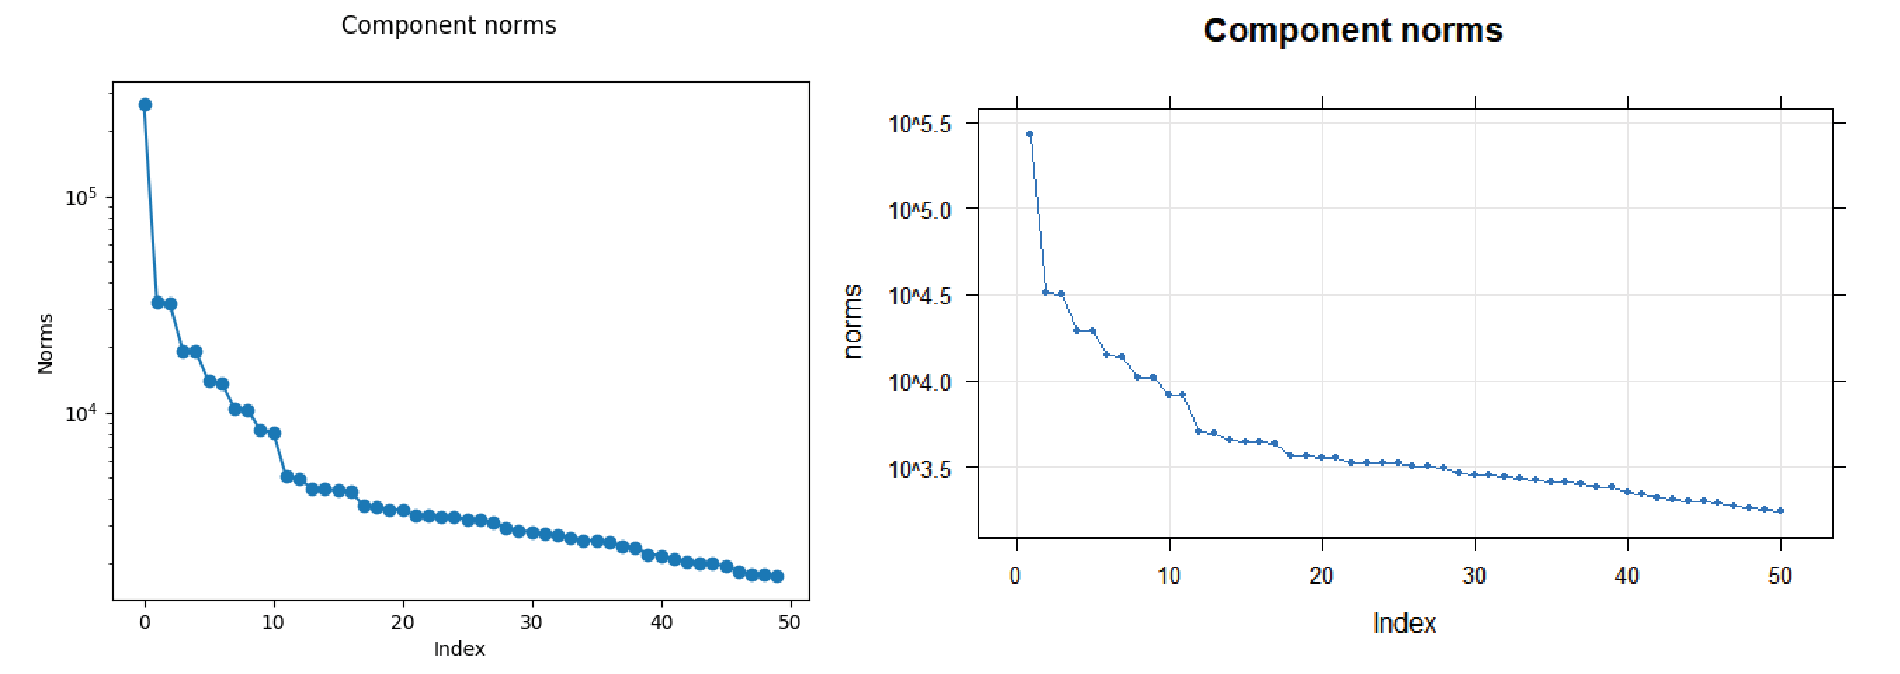
\includegraphics[width=0.65\textwidth]{rpy_norms}
	\caption{График норм компонент разложения в Python и R.}
	\label{fig:rpy_norms}
\end{figure}

\begin{figure}[htp]
	\centering
	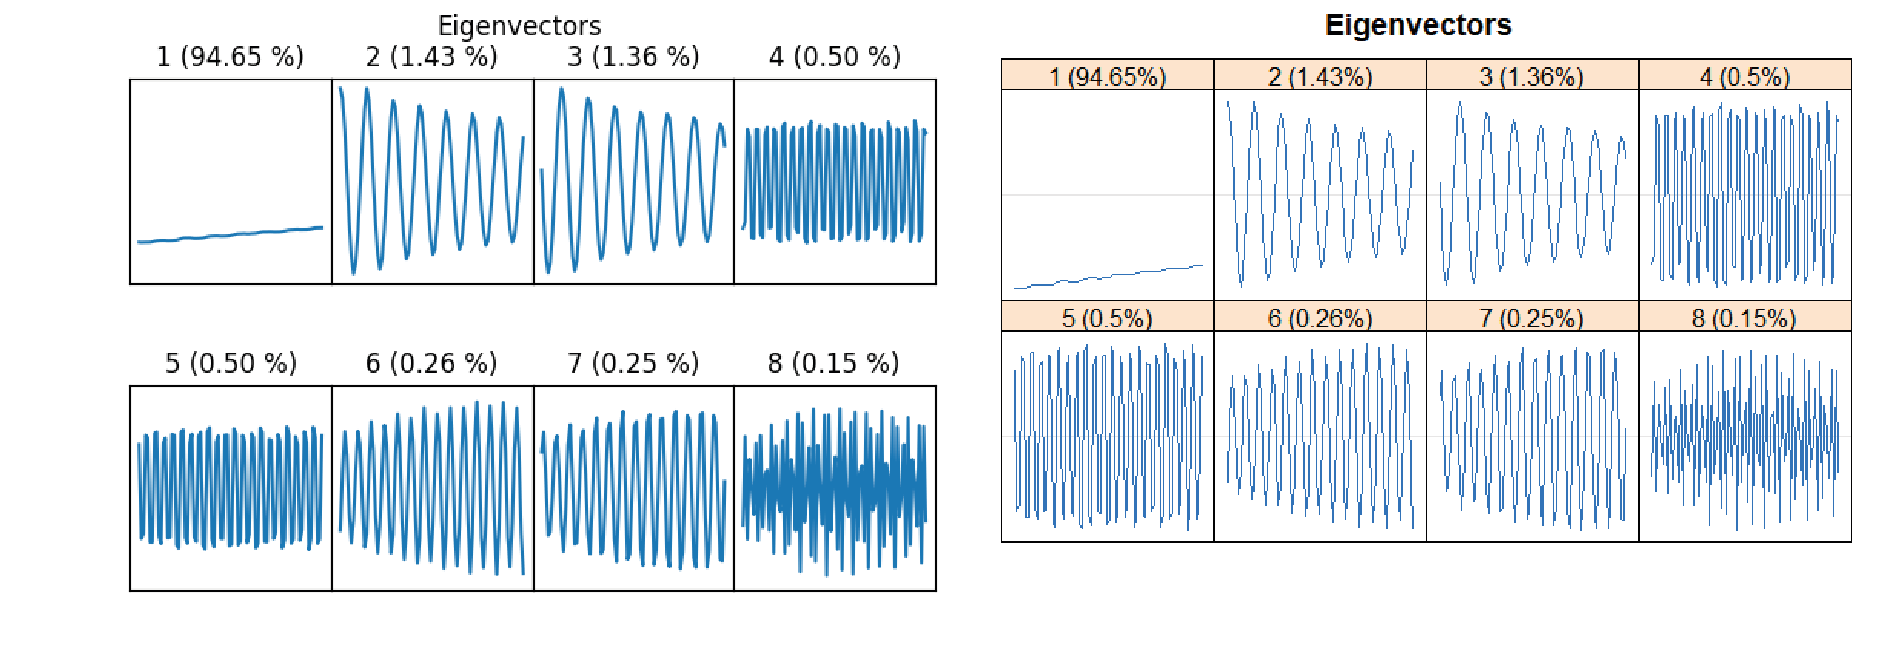
\includegraphics[width=0.65\textwidth]{rpy_vectors}
	\caption{График собственных векторов компонент разложения в Python и R.}
	\label{fig:rpy_vectors}
\end{figure}

\begin{figure}[htp]
	\centering
	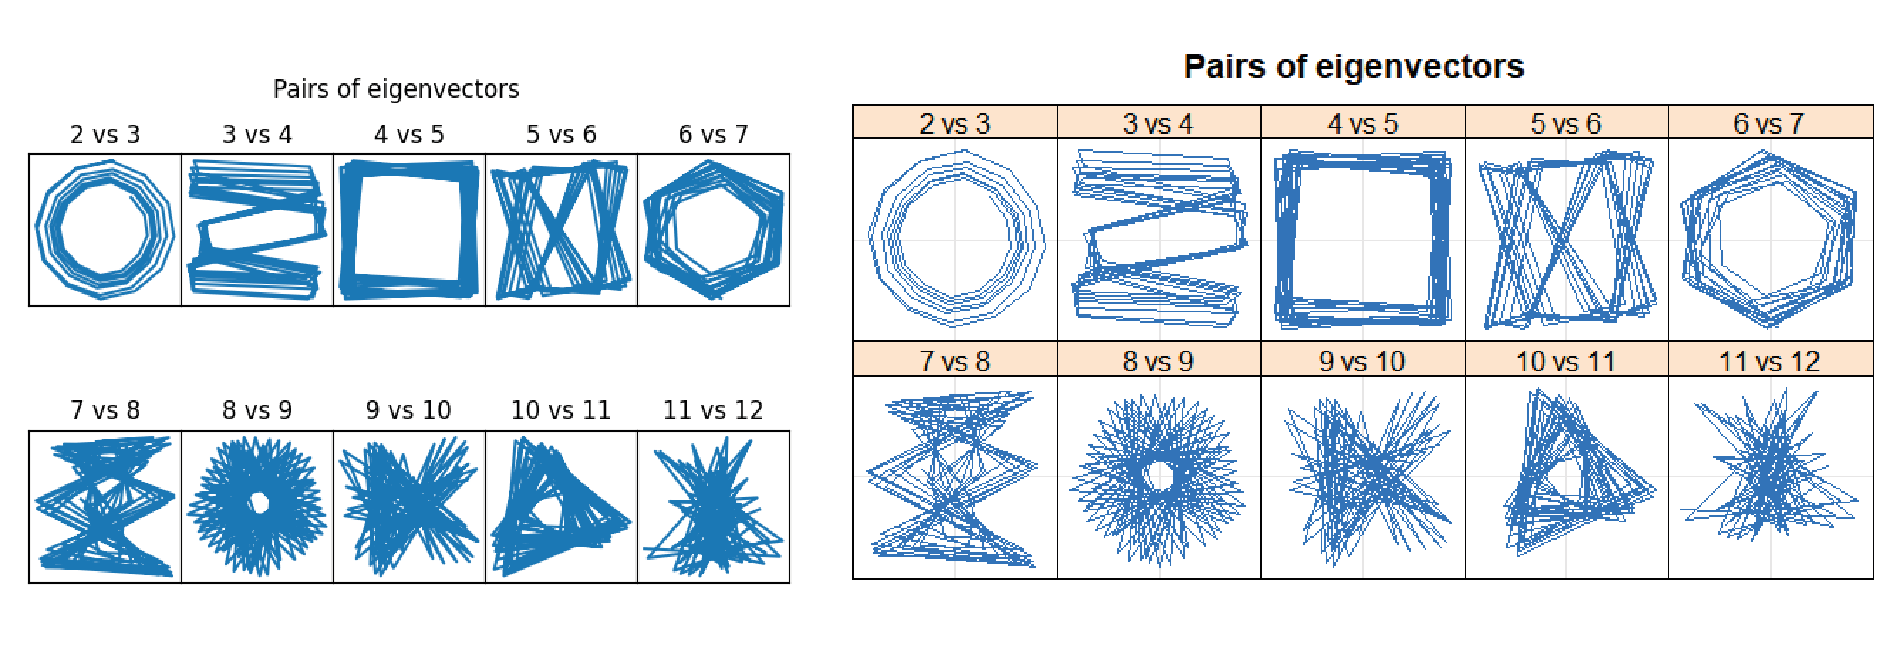
\includegraphics[width=0.65\textwidth]{rpy_pairs}
	\caption{Парный график собственных векторов компонент разложения в Python и R.}
	\label{fig:rpy_pairs}
\end{figure}

\begin{figure}[htp]
	\centering
	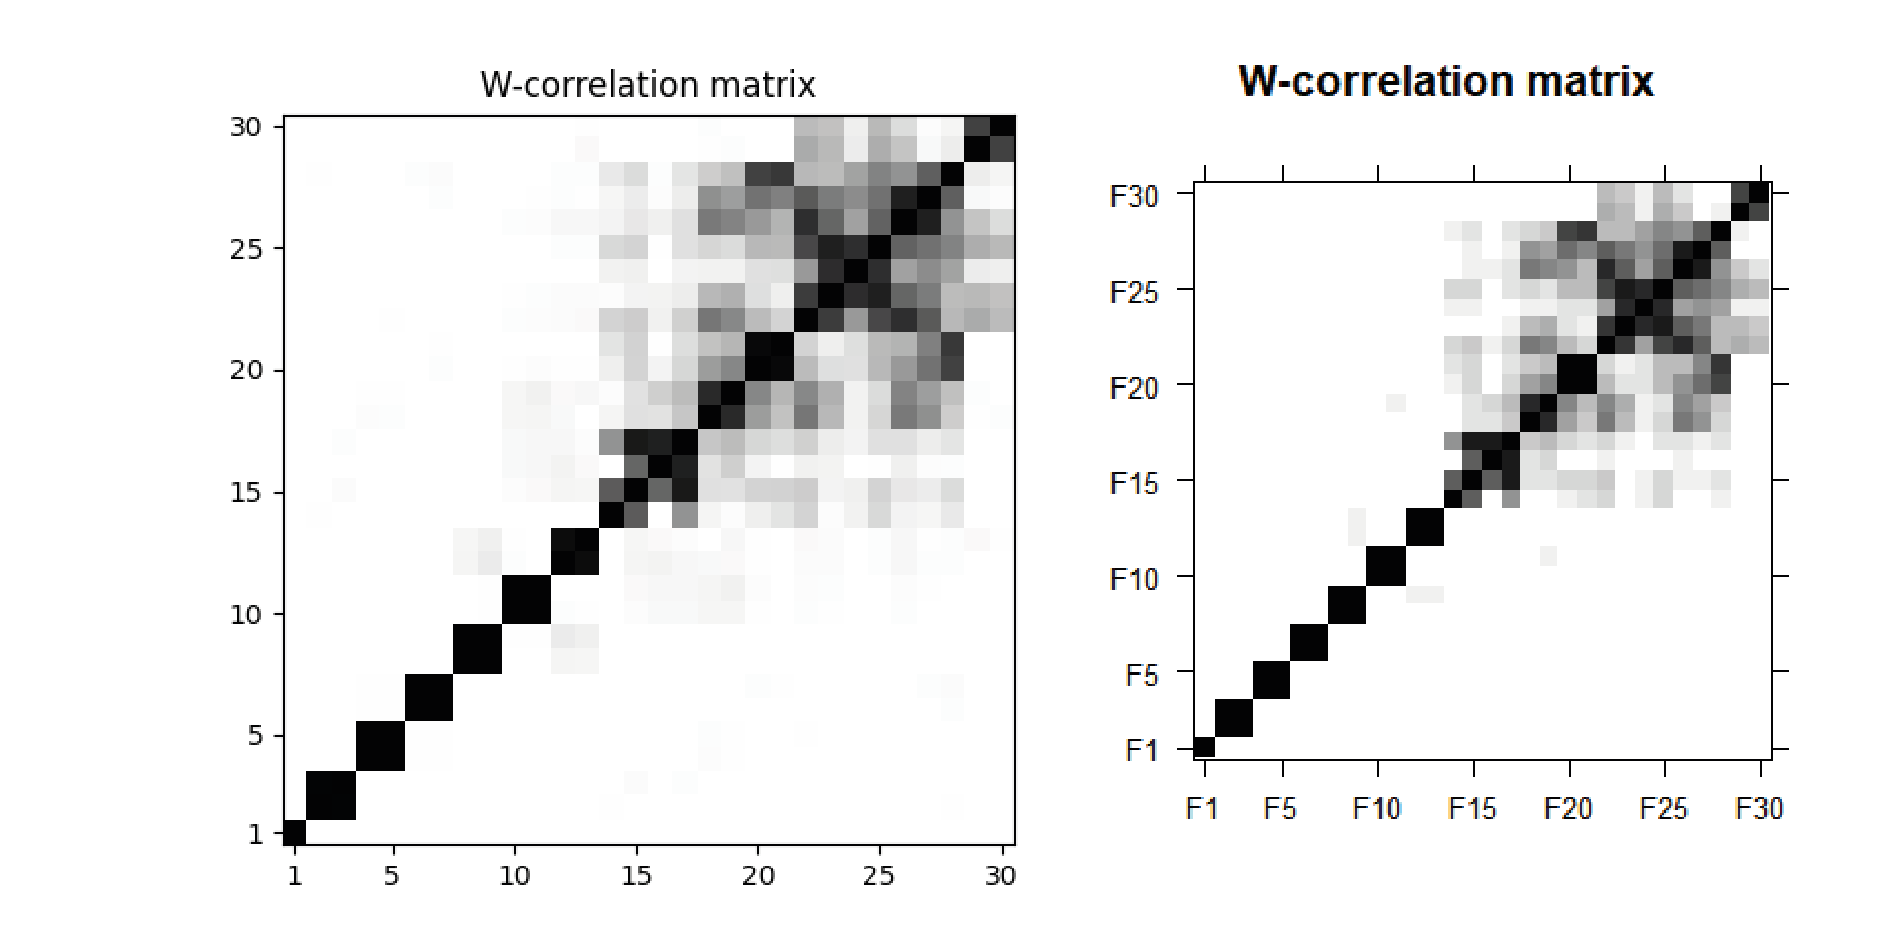
\includegraphics[width=0.65\textwidth]{rpy_wcor}
	\caption{График взвешенных корреляций компонент разложения в Python и R.}
	\label{fig:rpy_wcor}
\end{figure}

\subsection{Восстановление}

После первичного анализа разложения временного ряда и выбора компонент для восстановления исходного ряда, возникает необходимость в визуализации результатов восстановления. Функция отрисовки графиков имеет регулируемые параметры, позволяющие изображать полученное восстановление как на общем графике, так и на отдельных.

\begin{figure}[htp]
	\centering
	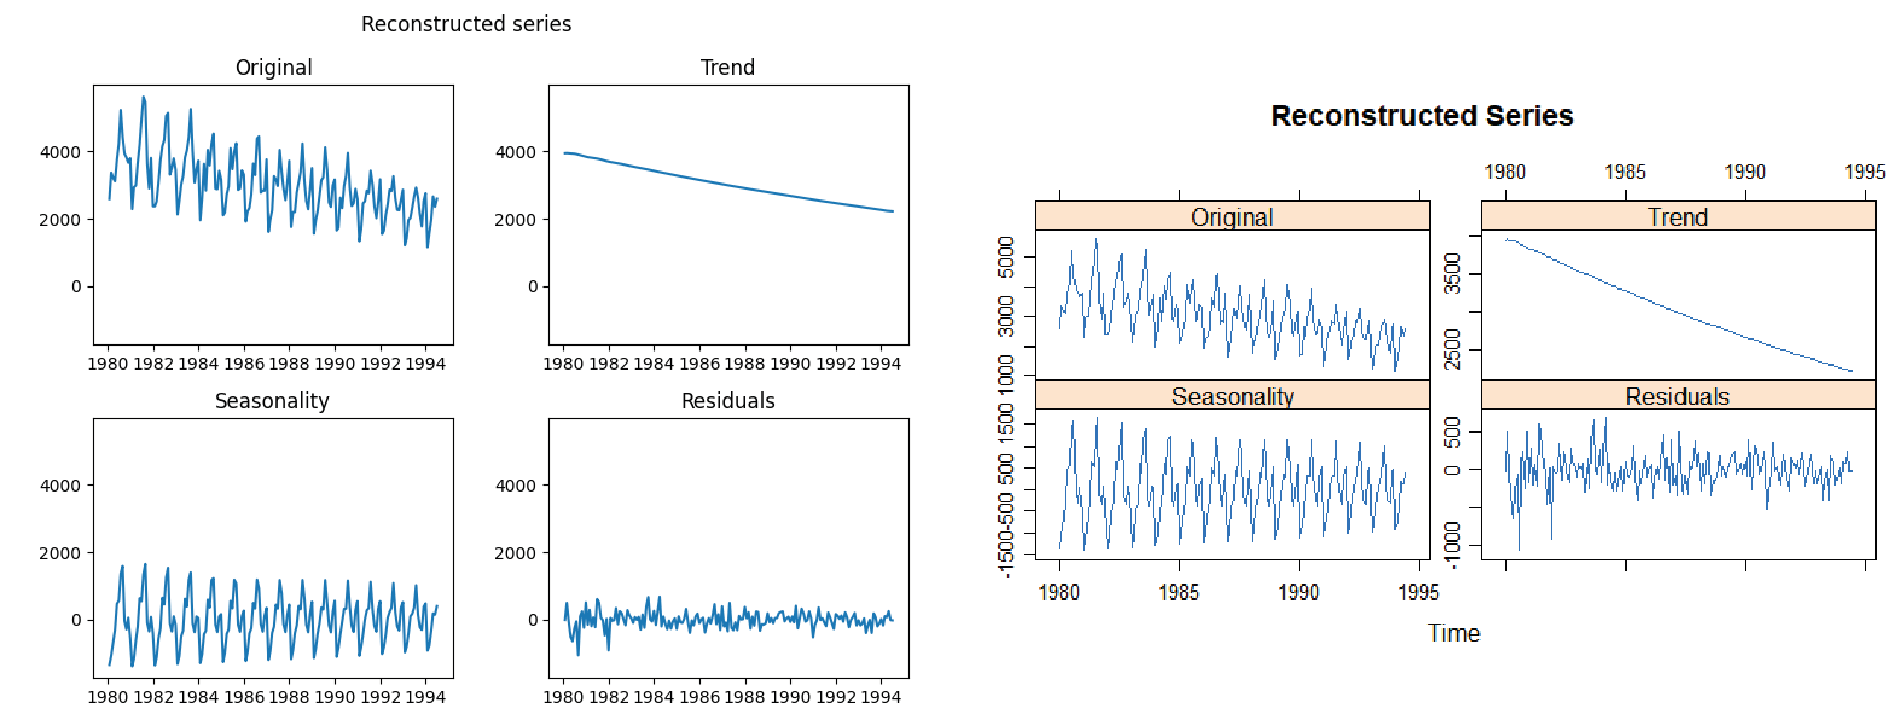
\includegraphics[width=0.65\textwidth]{rpy_rec}
	\caption{Визуализация восстановления на отдельных графиках в Python и R.}
	\label{fig:rpy_rec}
\end{figure}

\begin{figure}[htp]
	\centering
	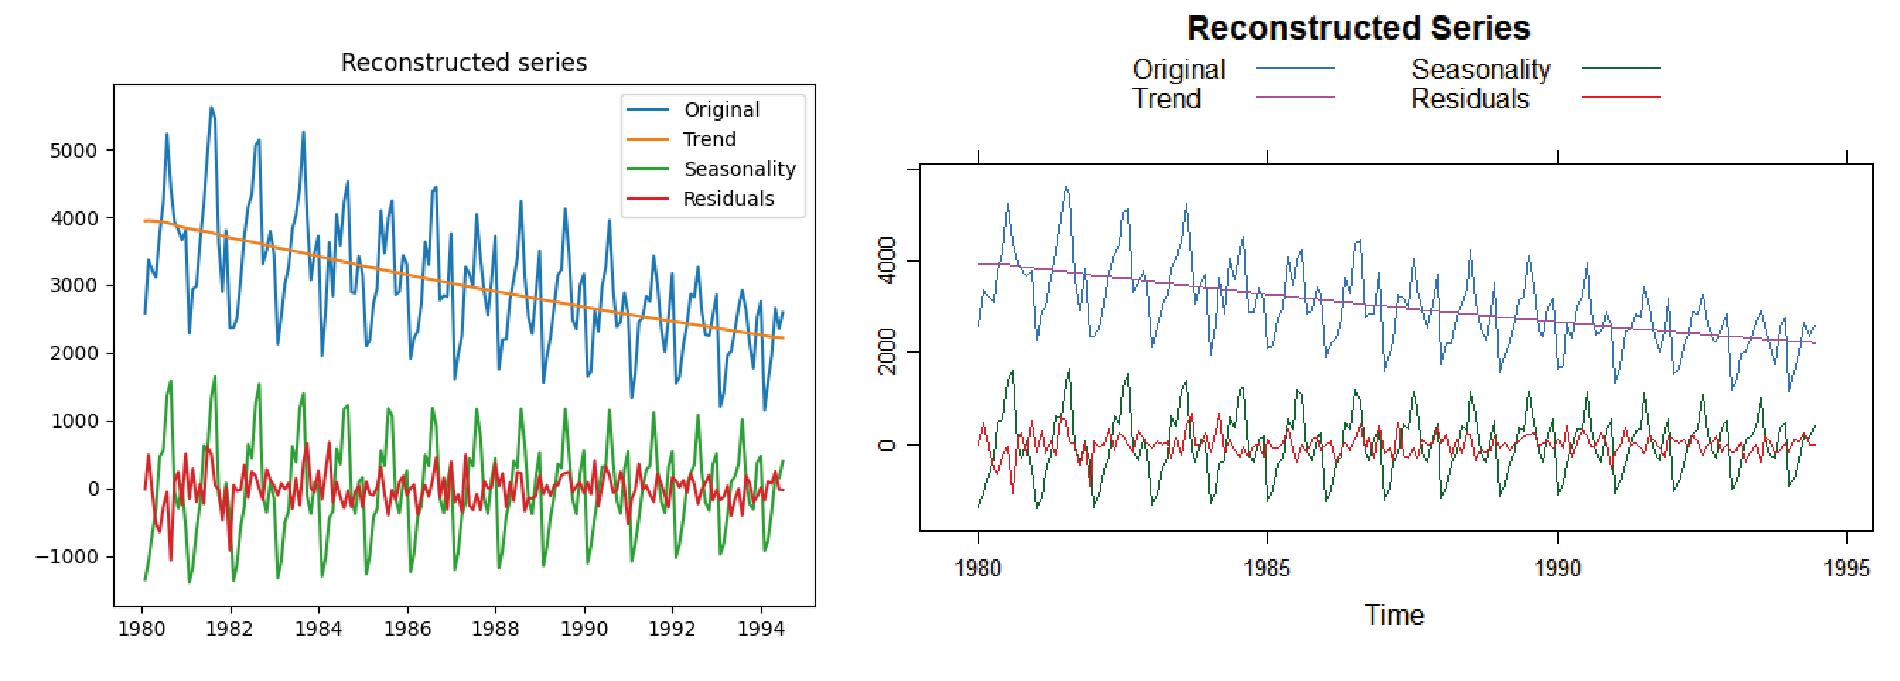
\includegraphics[width=0.65\textwidth]{rpy_rec_superpose}
	\caption{Визуализация восстановления на общем графике в Python и R.}
	\label{fig:rpy_rec_superpose}
\end{figure}

Реализованные на данный момент графики в будущем нуждаются в косметических доработках, изменениях и улучшениях, однако на данный момент они обладают достаточно хорошей информативностью для использования в исследованиях, а график взвешенных корреляций имеет даже более высокую детализацию по сравнению с аналогичным в R.

\section{Модельный пример}

Полученный в рамках задачи по адаптации модуля Rssa к языку Python результат может быть применен к какому-либо временному ряду. Для большей наглядности возьмем за основу модельный ряд, в котором будут присутствовать тренд, шум и сезонность. 

\begin{equation*}
	F_N = F_N^{(1)} + F_N^{(2)} + F_N^{(3)},
\end{equation*}
где $F_N^{(1)} = (f_1^{(1)}, \dots, f_{N}^{(1)}), f_n^{(1)} = 0.65 n$ – компонента ряда, содержащая тренд. $F_N^{(2)} = (f_0^{(2)}, \dots, f_{N-1}^{(2)}), f_n^{(2)} = \cos({2 \pi n \over 6})$ – компонента ряда, отвечающая за периодичность, а $F_N^{(3)} = (f_1^{(3)}, \dots, f_{N}^{(3)})$ – шум, где $f_n^{(3)}$ – независимые случайные величины, имеющие одно и то же нормальное распределение с нулевым средним и стандартным отклонением, равным $0.5$.

\begin{figure}[H]
	\centering
	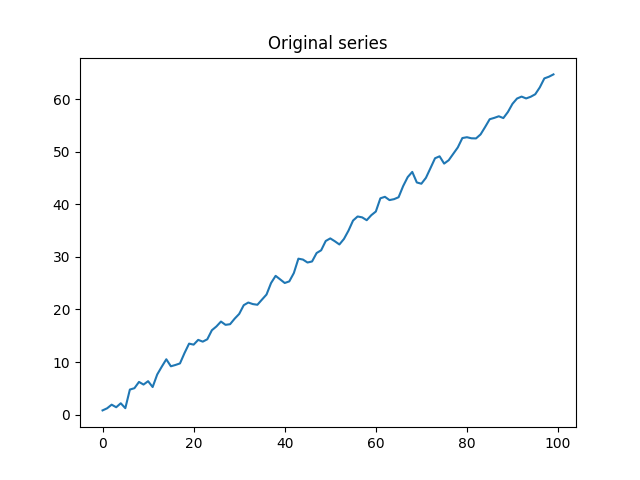
\includegraphics[width=0.5\textwidth]{mpy_orig}
	\caption{График исходного временного ряда.}
	\label{fig:mpy_orig}
\end{figure}

Далее, для разложения данного ряда на тренд, шум и периодичность, необходимо задать определенную длину окна. В связи с тем, что мы будем анализировать ряд базовым методом, нет смысла брать длину окна, большую, чем половина длины ряда. Таким образом, если $N = 100$, то $L \leq 50$.\\

Для разделения временного ряда на компоненты сперва обратимся к графикам полученных с помощью метода SSA собственных векторов.

\begin{figure}[H]
	\centering
	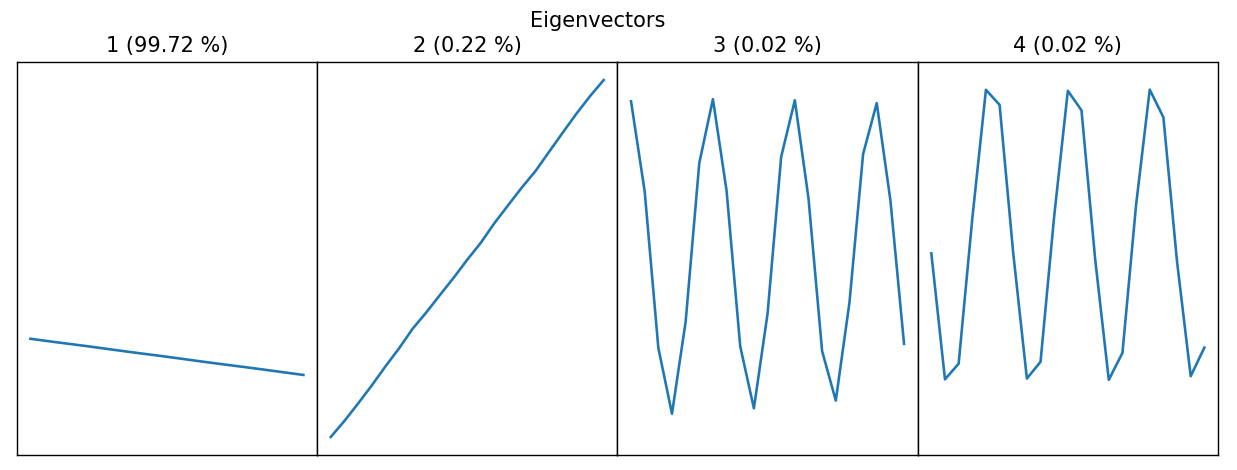
\includegraphics[width=0.5\textwidth]{mpy_vectors}
	\caption{Собственные векторы.}
	\label{mpy_vectors}
\end{figure}

В связи с тем, что в данном ряде тренд ярко выраженный, на первых позициях будет находиться большинство собственных векторов, соответствующих тренду. Таким образом, чтобы извлечь из имеющегося ряда тренд, необходимо собрать тройки, соответствующие медленно меняющимся сингулярным векторам. В данном случае, это первые два вектора.\\

Помимо этого необходимо выделить и сезонность. Третий и четвертый векторы имеют периодические колебания, в связи с чем для большей наглядности можно их сгруппировать и построить график.

\begin{figure}[H]
	\centering
	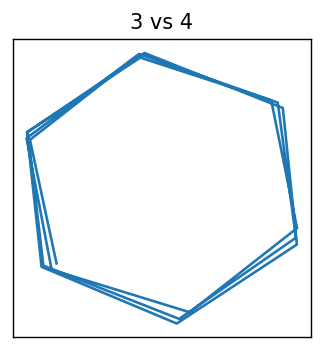
\includegraphics[width=0.25\textwidth]{mpy_pairs}
	\caption{Двумерная диаграмма пары векторов 3 и 4.}
	\label{mpy_pairs}
\end{figure}

Из данного графика достаточно хорошо видно, что период $T = 6$, так как на графике отчетливо виден шестиугольник. Это соответствует действительности, потому что в данном модельном ряде был выбран именно такой период. Далее построим реконструкцию ряда, где первая и вторая компоненты будут соответствовать тренду, а третья и четвертая – сезонности. 

\begin{figure}[H]
	\centering
	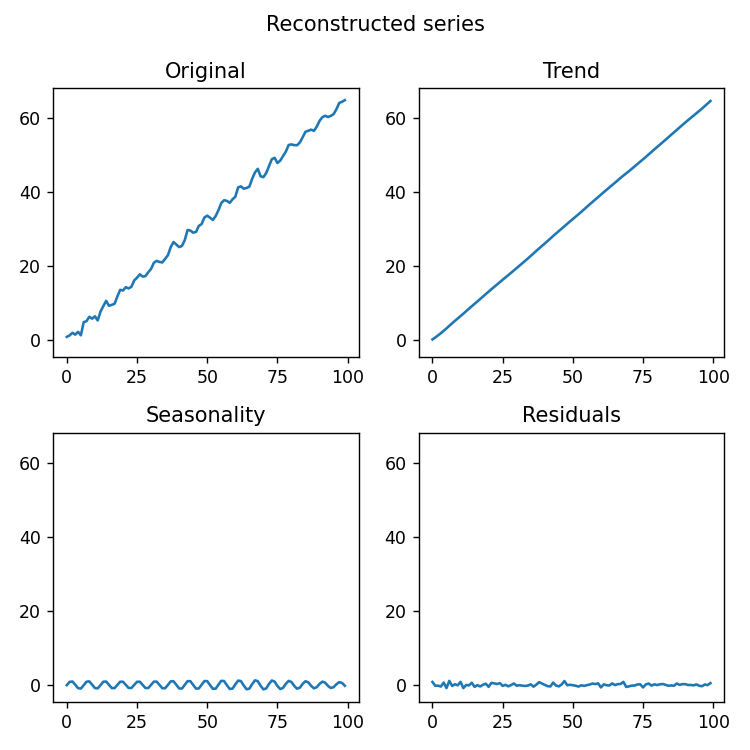
\includegraphics[width=0.6\textwidth]{mpy_rec}
	\caption{Реконструкция временного ряда.}
	\label{mpy_rec}
\end{figure}

С использованием средств визуализации в Python можем проверить качество получившегося разложения.

\begin{figure}[H]
	\centering
	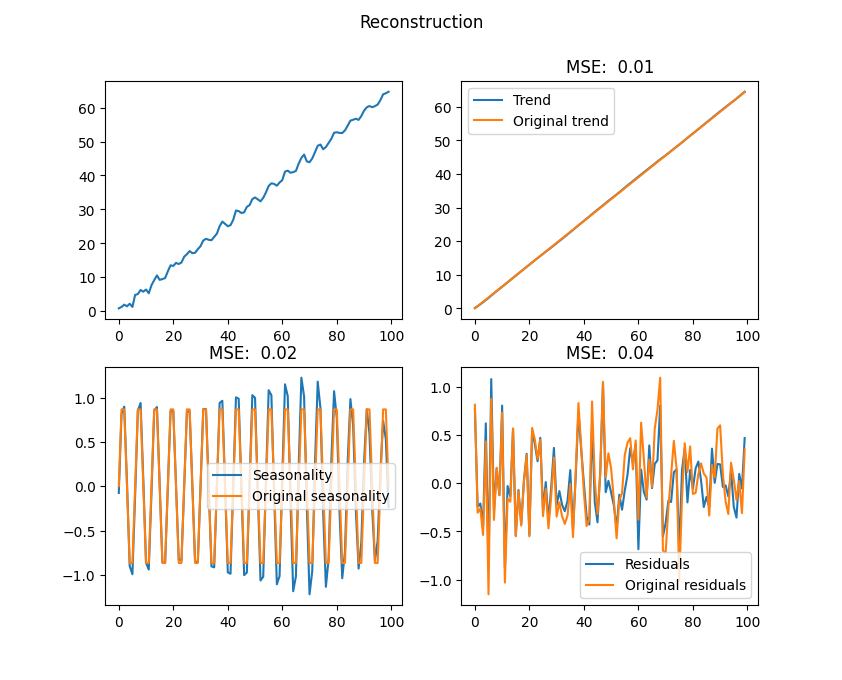
\includegraphics[width=0.6\textwidth]{mpy_tsr}
	\caption{Реконструкция модельного временного ряда.}
	\label{fig:mpy_tsr}
\end{figure}

Как видно из графиков, точность разложения достаточно высока, а тренд и сезонность определились практически идеально. Ниже приведен код, в результате которого удалось построить приведенные выше графики.

\begin{lstlisting}[language=Python, caption=Программный код для разложения и восстановления модельного ряда на Python.]
import pyrssa as prs
import numpy as np
import matplotlib.pyplot as plt
from sklearn.metrics import mean_squared_error as mse


np.random.seed(1)
N = 100
sigma = 0.5
noise = np.random.normal(size=N) * sigma
trend = 0.65 * np.arange(N)
seasonality = np.sin(2 * np.pi * np.arange(N) / 6)
series = seasonality + noise + trend

plt.plot(series)
plt.title("Original series")
plt.show()

s_series = prs.ssa(series, L=21, kind="1d-ssa")

prs.plot(s_series, kind="vectors", idx=range(1, 5))
prs.plot(s_series, kind="paired", idx=range(3, 5),
contrib=False)

r_series = prs.reconstruct(s_series,
groups={"Trend": range(1, 3),
	"Seasonality": range(3, 5)})
fig, ax = plt.subplots(2, 2)
fig.suptitle("Reconstruction")
ax[0, 0].plot(np.arange(N), series, label="Original")
ax[0, 1].plot(np.arange(N), r_series.Trend, label='Trend')
ax[0, 1].plot(np.arange(N), trend, label='Original trend')
ax[0, 1].set_title(
f"MSE: {mse(trend, r_series.Trend): .2f}")
ax[0, 1].legend()
ax[1, 0].plot(np.arange(N), r_series.Seasonality,
label='Seasonality')
ax[1, 0].plot(np.arange(N), seasonality,
label='Original seasonality')
ax[1, 0].set_title(
f"MSE: {mse(seasonality, r_series.Seasonality): .2f}")
ax[1, 0].legend()
ax[1, 1].plot(np.arange(N), r_series.residuals,
label='Residuals')
ax[1, 1].plot(np.arange(N), noise,
label='Original residuals')
ax[1, 1].set_title(
f"MSE: {mse(noise, r_series.residuals): .2f}")
ax[1, 1].legend()
plt.show()
\end{lstlisting}

Далее построим прогноз полученного модельного ряда.

\begin{lstlisting}[language=Python, caption=Программный код для прогноза модельного ряда на Python.]
for_length = 100
for_range = np.arange(N, N + for_length)
sigma = 0.5
for_trend = 0.65 * for_range
for_seasonality = np.sin(2 * np.pi * for_range / 6)
for_signal = for_seasonality + for_trend

rfor = prs.rforecast(s_series, groups={"Signal": range(1, 5)},
length=for_length)
plt.plot(for_signal)
plt.plot(rfor.Signal)
plt.legend(["Original series", "Forecasted series"])
plt.title(f"MSE: {mse(for_signal, rfor.Signal): .2f}")
plt.show()
\end{lstlisting}

Полученный результат приведен на графике ниже.

\begin{figure}[H]
	\centering
	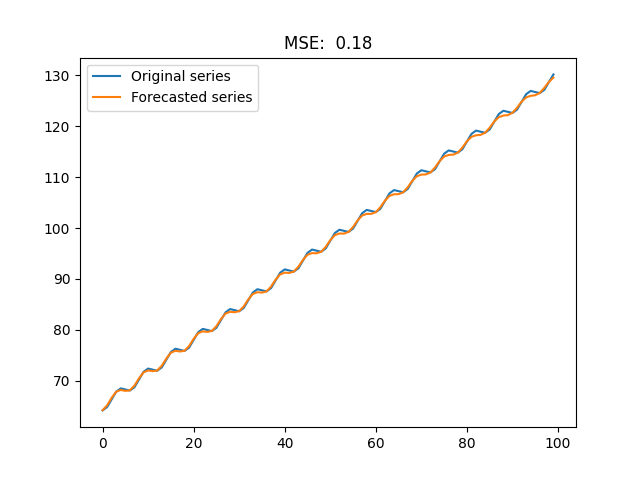
\includegraphics[width=0.5\textwidth]{mpy_for}
	\caption{Прогноз временного ряда.}
	\label{fig:mpy_for}
\end{figure}

\section{Установка модуля}

Как было сказано ранее, данный пакет опубликован на сайте проекта PyPi \cite{pyrssa-lib} и может быть установлен с помощью простой команды pip install pyrssa. При установке данного пакета автоматически подтягиваются зависимости, связанные с модулями NumPy, pandas, rpy2, matplotlib. Дополнительно проверяется наличие установленной библиотеки Rssa и в противном случае производится ее установка. Программный код, реализующий установку зависимостей, приведен ниже.

\begin{lstlisting}[language=Python, caption=Настройки проекта для публикации пакета на сайте PyPi.]
from setuptools import setup

setup(
name='pyrssa',
packages=['pyrssa', 'pyrssa.classes'],
include_package_data=True,
package_data={
	'data': ['*']},
version='1.0.6',
description='Rssa for Python',
license="Apache 2.0",
install_requires=['rpy2<=3.4.5', 'pandas', 
               'numpy', 'matplotlib'])
\end{lstlisting}

\begin{lstlisting}[language=Python, caption=Содержимое файла для инсталляции модуля Rssa.]
import rpy2.robjects.packages as rpackages
from rpy2.robjects.vectors import StrVector
utils = rpackages.importr('utils')
utils.chooseCRANmirror(ind=1)

def install_required():
	pack_names = ('Rssa',)
	names_to_install = [x for x in pack_names 
                  if not rpackages.isinstalled(x)]
	if len(names_to_install) > 0:
		utils.install_packages(
		StrVector(names_to_install))
\end{lstlisting}

На данный момент для пакета rpy2 обнаружены проблемы, начиная с версии 3.5.0, которые относятся к автоматическому приведению типов из R в Python, в связи с чем часть функциональности модуля теряется, поэтому на данный момент поставлено ограничение на версию модуля rpy2 вплоть до 3.4.5. Также, для того, чтобы модуль Rssa мог быть установлен, пользователь предварительно должен установить и настроить текущую версию языка R на своем устройстве, что является некоторым барьером в применении данного модуля.

\chapter{Анализ временного ряда}

\section{Исходные данные}

Исходными данными для анализа являются временные ряды параметров вращения Земли (ПВЗ), опубликованные Международной службой вращения Земли (МСВЗ) в бюллетене C04 \cite{eop-c04}. Описание рядов и процедур, используемых при обработке, приводится в \cite{eop-с04-guide}. Каждый из параметров измеряется ежедневно, за основу взята модифицированная юлианская дата (MJD), используемая Международным астрономическим союзом в качестве стандарта нумерации дней.\\

В рамках данной работы будет проанализирован ряд LOD (Length Of Day), который отражает разницу между фактическим временем полного оборота Земли вокруг своей оси и 86400 секундами. Ниже приведен график данного ряда.

\begin{figure}[H]
	\centering
	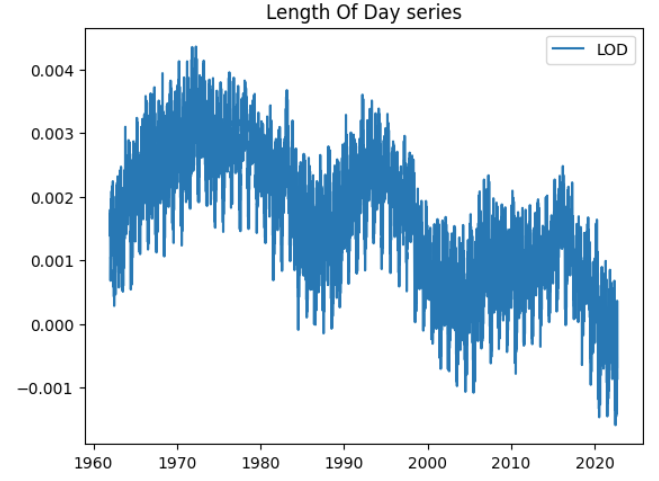
\includegraphics[width=0.6\textwidth]{py_lod_plot}
	\caption{График ряда долготы дня.}
	\label{fig:py_lod_plot}
\end{figure}

\section{Предварительный анализ ряда}

Сперва проанализируем ряд, оценив его параметры. Для анализа периодических составляющих ряда прибегнем к построению периодограммы, отражающей вклад различных частот в разложение Фурье исходного ряда. Построим графики с различными решетками частот для более наглядного выделения существующих пиков периодограммы.

\begin{figure}[H]
	\centering
	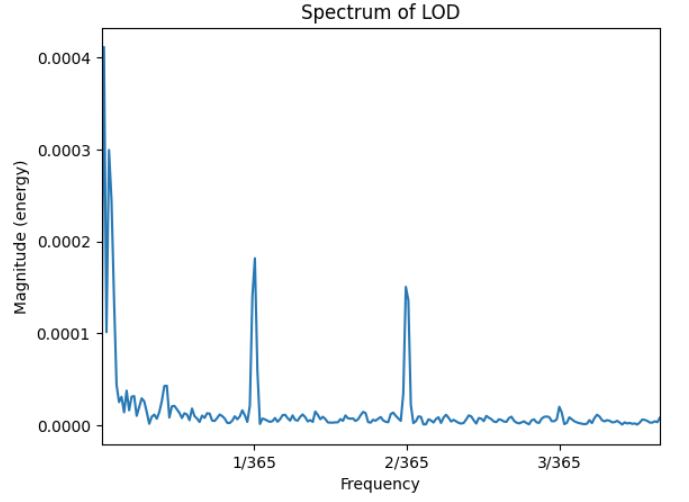
\includegraphics[width=0.6\textwidth]{py_lod_spec_365}
	\caption{Периодограмма ряда долготы дня для годовой решетки частот.}
	\label{fig:py_lod_spec_365}
\end{figure}

\begin{figure}[H]
	\centering
	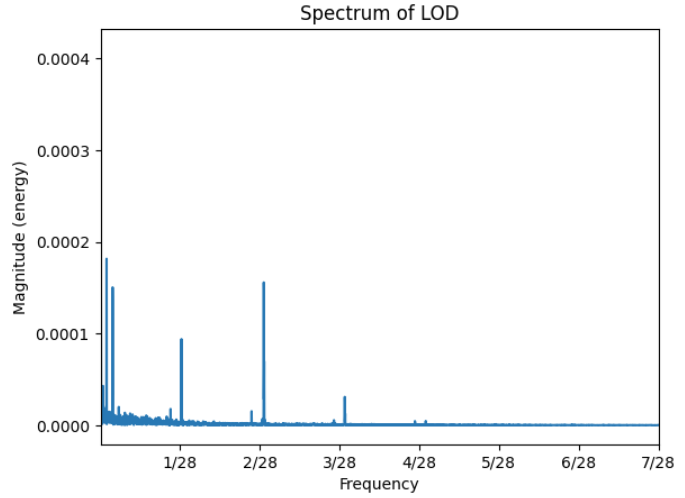
\includegraphics[width=0.6\textwidth]{py_lod_spec_28}
	\caption{Периодограмма ряда долготы дня для месячной решетки частот.}
	\label{fig:py_lod_spec_28}
\end{figure}


Как видно из графиков, периоды присутствующих в рядах гармоник приблизительно равны 365 и 28 дням. Рассмотрим базовое разложение SSA для данных рядов, отделив сезонные компоненты. 

\begin{figure}[H]
	\centering
	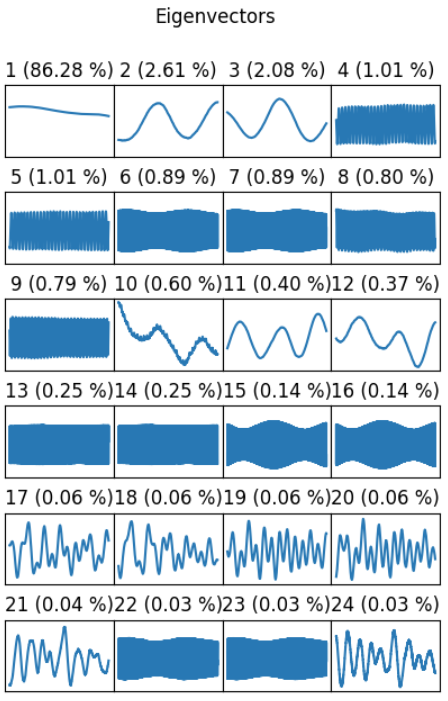
\includegraphics[width=0.4\textwidth]{py_lod_vectors}
	\caption{График собственных векторов разложения ряда долготы дня.}
	\label{fig:py_lod_vectors}
\end{figure}

\begin{figure}[H]
	\centering
	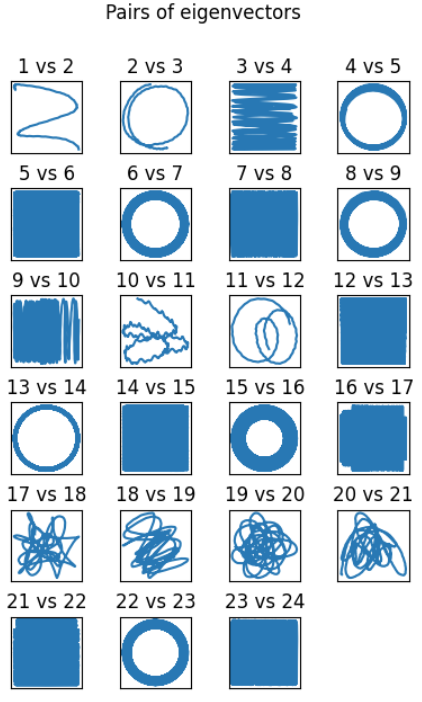
\includegraphics[width=0.4\textwidth]{py_lod_pairs}
	\caption{Парный график собственных векторов разложения ряда долготы дня.}
	\label{fig:py_lod_pairs}
\end{figure}

На графике векторов ряда долготы дня видны пары  4 и 5, 8 и 9, которые являются составляющими периода длиной в 365 дней, а также 6 и 7, 13 и 14, которые составляют период 28 дней. Оставшиеся пары также образуют один из двух указанных выше периодов.\\

\section{Подбор параметров для прогноза}

Для выбора параметров $L, r$ и метода прогнозирования при анализе ряда долготы дня прибегнем к перебору по сетке, рассмотрев все комбинации параметров $L = 300, 600, \dots, 3600$, $r = 1, \dots, 50$, а также рекуррентный и векторный метод прогноза.

В качестве меры ошибки будем использовать среднеквадратическую ошибку MSE (Mean Squared Error). Разделим ряд на несколько составляющих: базовый отрезок длиной в 15 лет, на основе которого строится разложение, валидационный отрезок длиной в 10 лет, который используется для оценки прогноза, а также тестовый отрезок длиной в один год, на котором полученный результат будет проверен впоследствии. Для наиболее качественного оценивания прибегнем к кросс-валидации, в рамках которой рассматриваемые базовый и валидационный отрезок будут смещаться по очереди 10 раз на один год вперед вплоть до начала тестового отрезка. Выбранные ранее параметры были предварительно оценены как оптимальные в другой работе, связанной с анализом данных рядов \cite{eop-analysis}. 

Результат данного алгоритма выведем с помощью объемного графика, по оси $x$ и $y$ которого находятся параметры $L, r$, а по оси $z$ изображено значение MSE. В связи с тем, что разница между некоторыми значениями составляет несколько порядков, данный график приведен в логарифмической шкале по оси $z$. Дополнительно с помощью цветовой карты от синего до красного цвета изображены лучшие и худшие значения среднеквадратической ошибки.

\begin{figure}[H]
	\centering
	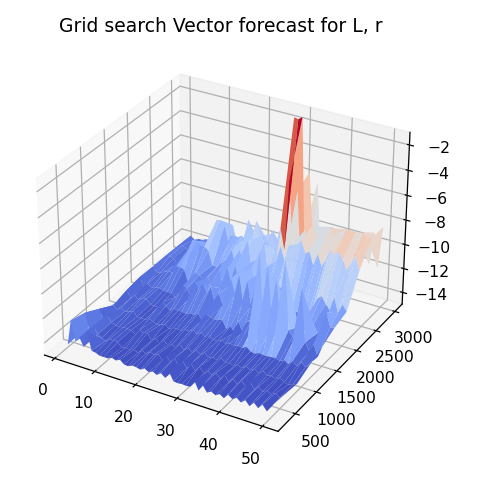
\includegraphics[width=0.5\textwidth]{py_lod_for_cv}
	\caption{График зависимости MSE от различных значений параметров L, r.}
	\label{fig:py_lod_for_cv}
\end{figure}

По данному графику видно, что наилучшее значение достигнуто для наименьшего по параметру $L = 300$, в связи с чем построим аналогичную сетку, выбрав параметр $L = 100, 200, \dots, 600$. 

\begin{figure}[H]
	\centering
	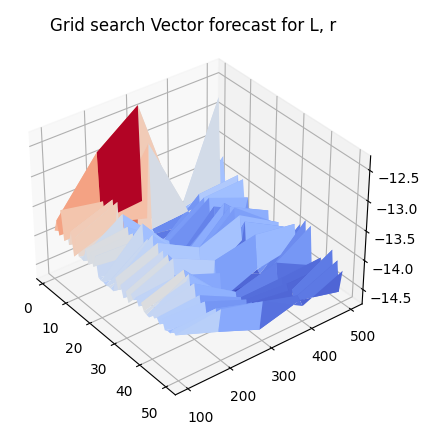
\includegraphics[width=0.5\textwidth]{py_lod_for_cv_2}
	\caption{График зависимости MSE от различных значений параметров $L, r$ на малой сетке по параметру $L$.}
	\label{fig:py_lod_for_cv_2}
\end{figure}

В связи с тем, что векторный прогноз показал более точные результаты при подборе параметров, остановимся на этом методе. Наименьшее значение MSE действительно оказалось достигнуто на параметрах $L = 300, r = 32$. Построим прогноз на основе данных параметров.

\begin{figure}[H]
	\centering
	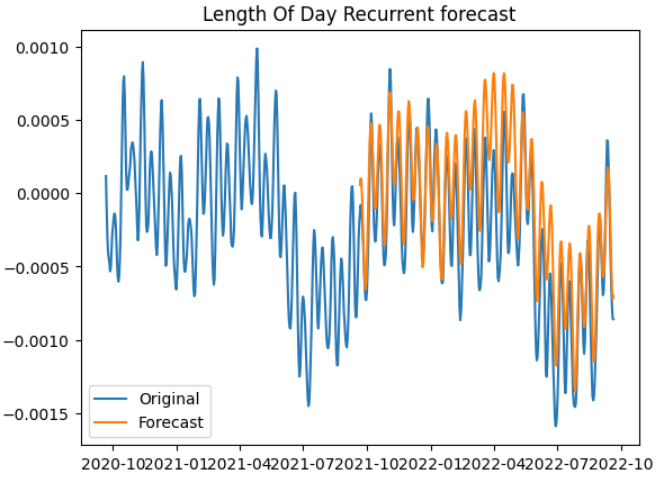
\includegraphics[width=0.6\textwidth]{py_lod_rec_min_res.png}
	\caption{График прогноза на основе подобранных параметров.}
	\label{fig:py_lod_rec_min_res}
\end{figure}

Полученный результат прогнозирования можно сравнить с прогнозом, полученным с помощью сайта \cite{eop-pred}, написанного в рамках указанной ранее работы \cite{eop-analysis}.

\begin{figure}[H]
	\centering
	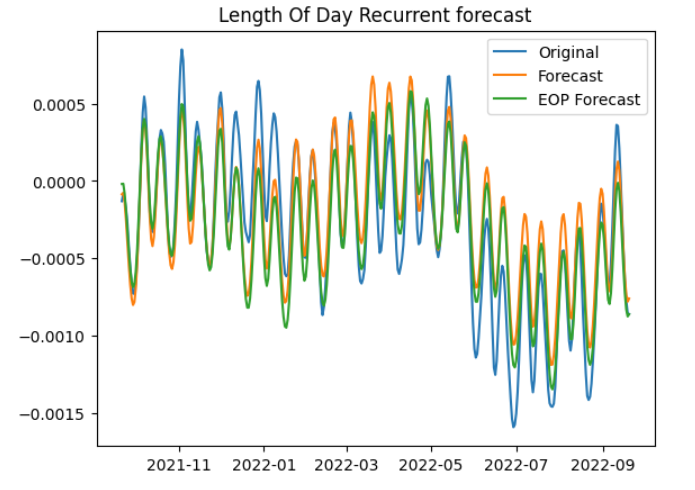
\includegraphics[width=0.6\textwidth]{py_lod_eop}
	\caption{График сравнения прогнозов временного ряда долготы дня.}
	\label{fig:py_lod_eop}
\end{figure}

Визуально данные прогнозы достаточно близки, в различных частях ряда каждый из прогнозов описывает значения лучше другого, а при проверке значений MSE можно заключить, что отличия у прогнозов минимальны: $6.6\text{e-}8$ для прогноза, полученного в рамках анализа, и $6.0\text{e-}8$ для прогноза с помощью сайта.

\chapter{Написание тестов для pyrssa}

Несмотря на то, что пакет pyrssa является адаптацией пакета Rssa, для которого уже существуют исчерпывающие тесты функциональности, для проверки правильности работы в рамках языка Python требуется портирование тестов и возможность проверки получаемых результатов, которые потенциально могут быть искажены при конвертации типов данных, а также в случае, если какие-либо функции пакета rpy2 не работают так, как это предполагается. 

\section{Загрузка данных}

Для тестов, используемых в пакете Rssa, были заранее сгенерированы эталонные данные, представляющие собой корректные результаты работы проверяемых функций. Для краткости описание структуры будет приведено к тестам, написанным для базового метода SSA. Хранение файлов организовано в формате .rda (R Data), который является форматом хранения данных в языке R, и в данном случае этот файл содержит различные временные ряды, для которых сосчитаны результаты работы функций при различных значениях параметра длины окна. Помимо этого, для них также указаны разные варианты группировки компонент, получаемых при разложении исходных рядов. Также для каждого из временных рядов дополнительно указаны параметры, содержащие название ряда, названия содержащихся в них результатов, наборы используемых значений параметра длины окна, группировки, указывается точность, с которой должны совпадать эталонные и получаемые значения, а также различные методы построения сингулярного разложения для рядов.

Для наглядности работы и возможности внесения корректировок в рамках языка Python реализована структура хранения данной информации в различных папках. Таким образом, в корневой папке для тестов находится дочерняя директория, содержащая данные, внутри которой идет подразделение на виды проверок, для каждого из видов созданы директории под различные длины окна, а внутри них в формате .csv собраны таблицы, столбцы которых состоят из результатов различных вариантов группировки компонент. Хранение дополнительных параметров организованы в формате JSON. Примерное содержание такого файла указано в листинге ниже.

\begin{lstlisting}[language=Python, caption=Содержимое файла JSON с параметрами для тестов.]
{
	"name": "co2",
	"names": ["series", "reconstruction",
	  "rforecast.orig", 
	  "rforecast.rec", "vforecast"],
	"what": ["reconstruct", "rforecast", "vforecast"],
	"kind": "1d-ssa",
	"Ls": 
	 	{"reconstruct":  [17, 234, 235, 300, 400],
	 "forecast":  [17, 100, 222, 234]},
	"groups": 
  {"reconstruct": [[1], [2], [3], [4], ...],
		"forecast":  [[1], [1, 2], [3, 4, 5], ...]},
	"len": 100,
	"neig": 20,
	"tolerance": 2e-07,
	"svd_methods": 
		{"reconstruct": [
			["svd", "eigen", "propack"]],
	 "forecast": [
			["svd", "eigen", "propack"]]}
}
\end{lstlisting}

После обновления структуры хранения данных для тестов также возникла необходимость в их корректном считывании при загрузке в Python. Для решения этой задачи были также реализованы специальные функции. Код для этих функций приведен ниже за исключением значений некоторых параметров и кода иных функций, которые в целом не влияют на основную логику.

\begin{lstlisting}[language=Python, caption=Функции для загрузки данных для тестирования.]
	
def load_df(df_name, kinds: list, file_format="csv"):
 filename = os.path.join(TEST_DATAFRAME_DIRECTORY,
                         df_name)
    print(filename)
    if kinds is None:
        kinds = os.listdir(filename)
    data_folders = [
    [os.path.join(filename, name), name]
    for name in kinds
    if os.path.isdir(os.path.join(filename, 
                                  name))]
    df = {"series": 
        pd.read_csv(
            os.path.join(
                filename, 
                f"series.{file_format}")),
          "pars": None}
	
	params_path = os.path.join(filename,
                         "pars.json")
	if os.path.exists(params_path):
	df["pars"] = read_json(params_path)
	
	for data_folder in data_folders:
	folder_files = [
  [os.path.join(data_folder[0], file), file]
  for file in os.listdir(data_folder[0])]
	df[data_folder[1]] = {
     file[1].replace(f".{file_format}", ""):
     pd.read_csv(file[0])
     for file in folder_files}
    return df


def load_dataframes(df_names=DATAFRAME_NAMES, 
kinds=DATAFRAME_KINDS):
	return {df_name: load_df(df_name, kinds=kinds) 
			for df_name in df_names}
\end{lstlisting}

\section{Тестирование}

После загрузки данных следующей задачей становится их непосредственное тестирование. Для упрощения и автоматизации части процессов за основу был взят стандартный для Python модуль unittest \cite{unittest-doc}, поставляемый вместе с программной оболочкой языка. Удобство данного модуля заключается также и в том, что с его помощью можно быстро запускать тесты в продвинутых средах разработки, имея возможность посмотреть на результаты каждого из тестов без необходимости в изучении лишь отладочной информации. Однако, при решении задачи написания тестов возникли сложности с тем, что встроенной поддержки сравнения табличных данных данный пакет не имеет, а визуальное восприятие больших объемов кода было затруднено. В связи с этим тестирование посредством модуля unittest и действительное сравнение значений были вынесены в различные места. Далее будут приведены выдержки, относящиеся к каждой из тестируемых функций.

\subsection{Восстановление}

Для проведения тестов на восстановление временного ряда предварительно строится его разложение на компоненты, а затем с учетом параметров тестирования происходит подсчет необходимых значений. Ниже приведены листинги, относящиеся к тестированию правильности восстановления временных рядов.
 
\begin{lstlisting}[language=Python, caption=Функции для подсчета значений восстановления временного ряда при тестировании.]
	
def compute_reconstructions(
                x, Ls, groups,
                kind: Literal["1d-ssa", "toeplitz-ssa"] = "1d-ssa",
                svd_method: Literal["auto", "eigen", 
                                    "propack", "nutrlan",
                                    "svd"] = "auto",
                neig=None,
                column_projector="none",
                row_projector="none",
                **kwargs):
    if neig is None:
        if isinstance(groups, dict):
            neig = np.max(list(chain(*groups.values())))
        elif isinstance(groups, list):
            neig = np.max([np.max(i) for i in groups])
        else:
            raise TypeError(f"Wrong type for groups: 
                             {type(groups)}")

    def compute_reconstruction(L):
        ss = prs.ssa(x, L, kind=kind, svd_method=svd_method,
                     neig=min(neig, L),
                     column_projector=column_projector,
                     row_projector=row_projector,
                     **kwargs)
        rec = prs.reconstruct(ss, groups=groups)
        return pd.DataFrame({key: rec[key] for key in rec.names})

    return {f"L{L_value}": compute_reconstruction(L_value)
    	    for L_value in Ls}

\end{lstlisting}

Тестирование функций подразумевает перебор различных параметров для получения результатов. В силу большого объема функции, в которой производится тестирование, фрагмент, относящийся к инициализации параметров будет опущен, и далее приведены лишь выдержки кода, производящие перебор по параметрам.

\begin{lstlisting}[language=Python, caption=Перебор параметров восстановления и проверка результатов на правильность.]
	
for i in range(len(Ls)):
    L = Ls[i]
    L_name = f"L{L}"
    for svd_method in svd_methods[i]:
        print(f"Data: {name},
                Kind: {kind}, 
                SVD-Method: {svd_method},
                L: {L}...", end="")
    reconstruction = 
        compute_reconstructions(series, [L], 
                                groups=groups, 
                                kind=kind, 
                                svd_method=svd_method,
                                neig=neig, 
                                column_projector=column_projector,
                                row_projector=row_projector)
    pd.testing.assert_frame_equal(
        reconstruction[L_name], 
        test_data["reconstruction"][L_name],
        rtol=tolerance)
    print("OK")
	
\end{lstlisting}

Описанный в листинге выше код выполняет перебор значений параметра длины окна, а также для каждого из них перебор различных методов построения сингулярного разложения. Для каждой комбинации параметров строится свое разложение и затем с помощью функции пакета pandas, позволяющей сравнивать наборы данных, производится сравнение значений с заданной точностью. В случае, если возникают отличия, функция проверки выбрасывает исключение. Ниже приведен код, относящийся к запуску тестов и обработке возникющих исключений.

\begin{lstlisting}[language=Python, caption=Запуск тестов правильности восстановления временного ряда и обработка исключений.]

import unittest
from tests.tests_methods import test_test_data, all_test_data


class Test1DSSA(unittest.TestCase):

    def test_reconstruct(cls):
        what = "reconstruct"
        names = ["co2", "fr1k.nz", "fr1k", "fr50", "fr50.nz"]
        for name in names:
            try:
                test_test_data(what, all_test_data[name])
            except:
                cls.fail("Wrong result")
	
\end{lstlisting}

В приведенном фрагменте кода производится наследование класса TestCase модуля unittest, благодаря чему при запуске тесты автоматически подгружаются и поочередно запускаются. При этом, с использованием конструкции try-except обрабатывается исключение, в случае возникновения которого дальнейшее проведение тестов для текущей функции останавливается и производится переход к следующим функциям.


\subsection{Прогнозирование}

Тестирование производится как для рекуррентного, так и для векторного методов прогнозирования, однако, в связи с практически идентичной логикой программного кода, в некоторых случаях приведены будут лишь фрагменты, относящиеся к рекуррентному варианту. Стоит отметить лишь одно существенное отличие: рекуррентный прогноз может быть построен по значениям как исходного ряда, так и восстановленного, в то время, как векторный прогноз основывается лишь на полученных в результате разложения результатах. В листинге ниже приведена функция подсчета результатов прогнозирования для обоих методов в зависимости от значения параметра метода прогноза.

\begin{lstlisting}[language=Python, caption=Функции для подсчета значений прогноза временного ряда при тестировании.]

def compute_forecasts(
                 x, Ls, groups, length,
                 kind: Literal["1d-ssa", "toeplitz-ssa"] = "1d-ssa",
                 forecast_method: Literal["recurrent", 
                                          "vector"] = "recurrent",
                 base: Literal["reconstructed", 
                               "original"] = "reconstructed",
                 svd_method: Literal["auto", "eigen", 
                                     "propack", "nutrlan",
                                     "svd"] = "auto",
                 neig=None,
                 column_projector="none",
                 row_projector="none",
                 **kwargs):
                 
    if neig is None:
        if isinstance(groups, dict):
            neig = np.max(list(chain(*groups.values())))
        elif isinstance(groups, list):
            neig = np.max([np.max(i) for i in groups])
        else:
            raise TypeError(f"Wrong type for groups: {type(groups)}")

    def compute_forecast(L):
        ss = prs.ssa(x, L, kind=kind, svd_method=svd_method,
                     neig=min(neig, L),
                     column_projector=column_projector,
                     row_projector=row_projector,
                     **kwargs)
        if forecast_method == "recurrent":
            rec = prs.rforecast(ss, groups=groups,
                                length=length, base=base,
                                only_new=False)
        else:
            rec = prs.vforecast(ss, groups=groups, 
                                length=length, only_new=False)

        return pd.DataFrame({key: rec[key] for key in rec.names})

    return {f"L{L_value}": compute_forecast(L_value)
    	    for L_value in Ls}
	
\end{lstlisting}


\begin{lstlisting}[language=Python, caption=Перебор параметров рекуррентного прогнозирования и проверка результатов на правильность.]
	
for i in range(len(Ls_forecast)):
    L = Ls_forecast[i]
    L_name = f"L{L}"
    for svd_method in svd_methods[i]:
        print(f"Data: {name},
                Kind: {kind}, 
                SVD-Method: {svd_method}, 
                L: {L}...", end="")
        rforecast_orig = 
            compute_forecasts(series,
                              [L], 
                              groups=forecast_groups,
                              length=length,
                              kind=kind,
                              forecast_method="recurrent", 
                              base="original",
                              svd_method=svd_method, 
                              neig=neig,
                              column_projector=column_projector, 
                              row_projector=row_projector,
                              **kwargs)
        rforecast_rec = 
            compute_forecasts(series,
                              [L], 
                              groups=forecast_groups, 
                              length=length,
                              kind=kind, 
                              forecast_method="recurrent",
                              base="reconstructed",
                              svd_method=svd_method, 
                              neig=neig,
                              column_projector=column_projector, 
                              row_projector=row_projector,
                              **kwargs)

        pd.testing.assert_frame_equal(
            rforecast_orig[L_name],
            test_data["rforecast.orig"][L_name],
            rtol=tolerance)
        pd.testing.assert_frame_equal(
            rforecast_rec[L_name], 
            test_data["rforecast.rec"][L_name],
            rtol=tolerance)
        print("OK")
	
\end{lstlisting}

\begin{lstlisting}[language=Python, caption=Запуск тестов правильности рекуррентного прогнозирования временного ряда и обработка исключений.]
	
import unittest
from tests.tests_methods import test_test_data, all_test_data


class Test1DSSA(unittest.TestCase):
    def test_rforecast(cls):
        what = "rforecast"
        names = ["co2", "fr1k.nz", "fr1k", "fr50", "fr50.nz"]
        for name in names:
            try:
                test_test_data(what, all_test_data[name])
            except:
                cls.fail("Wrong result")
	
\end{lstlisting}

В рамках тестирования функций восстановления и прогнозирования были выявлены и устранены проблемы, связанные с обработкой параметров при их передаче в rpy2, однако дальнейшее тестирование может выявить иные проблемы, которые также потребуют корректировки работы некоторых функций.

\chapter{Сравнение скорости Rssa и pyrssa}
	
При использовании пакета Rssa в качестве основы для реализации метода SSA на языке Python одной из важнейших характеристик является скорость, а если быть точнее, то ее сохранение близкой к исходной. Для полноценного анализа скорости работы возьмем за основу ранее рассмотренный ряд длины дня из набора данных ПВЗ. Замер времени работы будет проводиться при различных комбинациях параметров $L$ длины окна и $r$ количества компонент, на основе которых сначала строилось разложение SSA, а затем восстановление ряда. Программный код для обоих языков программирования приведен ниже.

\begin{lstlisting}[language=R, caption=Программный код для анализа времени работы на языке R.]
L_range <- seq(from=300, to=3000, by=300)
r_range <- 1:50	

ssa_check <- function(time_series, L, r) {
	
	time_series_ssa <- ssa(time_series, L=L)
	ser_rec <- reconstruct(time_series_ssa,
	                       groups=list("Signal"=1:r))
	return(ser_rec)
	
}

for (L_value in L_range) {
	for(r_value in r_range) {
		time_df[r_value, as.character(L_value)] <- 
		system.time(ssa_check(series, L_value, r_value))[3]
	}
}
\end{lstlisting}

\begin{lstlisting}[language=Python, caption=Программный код для анализа времени работы на языке Python.]
import time
time_df = []

L_range = range(300, 3001, 300)
r_range = range(1, 51)

for r_value in r_range:
	cur_time = []
	for L_value in L_range:
		start_time = time.time()
		check_ssa(lod_series, L_value, r_value)
		check_time = time.time() - start_time
		cur_time.append(check_time)
time_df.append(cur_time)
\end{lstlisting}

В результате работы получена большая таблица данных, для более удобного визуального восприятия ниже приведены графики для параметров $L = 300, 1500, 3000$, где по оси $x$ варьируется число $r$ компонент для восстановления, а по оси $y$ изображено время, затраченное на выполнение разложения и восстановления.

\begin{figure}[H]
\centering
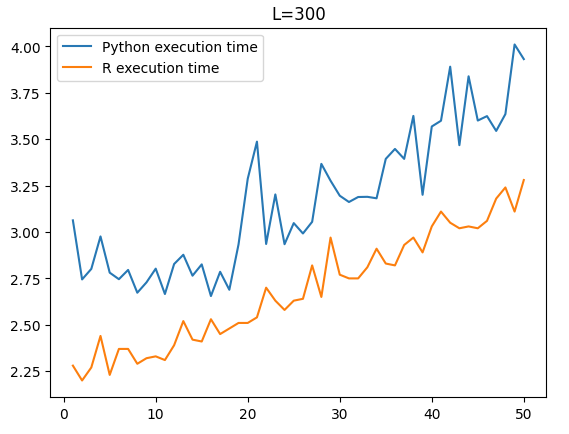
\includegraphics[width=0.45\textwidth]{time_test_L_300.png}
\caption{График затраченного времени для L=300.}
\label{fig:time_test_L_300}
\end{figure}

\begin{figure}[H]
	\centering
	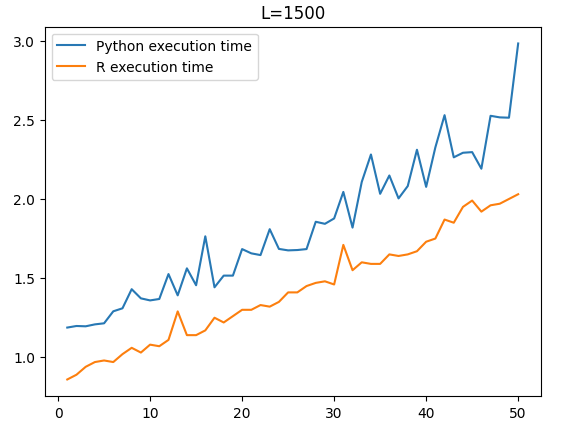
\includegraphics[width=0.45\textwidth]{time_test_L_1500.png}
	\caption{График затраченного времени для L=1500.}
	\label{fig:time_test_L_1500}
\end{figure}

\begin{figure}[H]
	\centering
	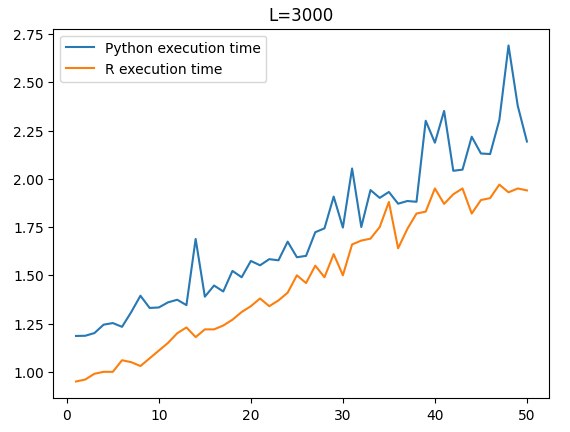
\includegraphics[width=0.45\textwidth]{time_test_L_3000.png}
	\caption{График затраченного времени для L=3000.}
	\label{fig:time_test_L_3000}
\end{figure}

Из данных графиков видно, что используемое в языке Python дополнительное время отличается на некоторый константный промежуток времени, который логично возникает из переводов типов данных между языками и дополнительных операций. В среднем данный промежуток составил 0.35 секунды, что в рамках данного ряда в процентном соотношении составляет порядка 15-20\%. Таким образом, в дальнейшем стоит задача максимально сократить это время.

\chapter{Заключение}

В рамках данной работы были рассмотрены уже существующие реализации метода SSA для языка Python, изучены различные особенности пакета Rssa, а также реализована часть методов и примеров применения данного пакета.

Помимо адаптации модуля Rssa к языку Python, удалось применить модуль matplotlib для визуализации результатов, заменив тем самым встроенные в R средства отрисовки графиков, обращение к которым в связи с особенностями для пакета Rssa было осложнено.

Также с помощью модулей unittest и pandas были адаптированы тесты для проверки результатов функций восстановления и прогнозирования временных рядов, позволившие выявить и устранить часть существующих проблем.

Реализованный пакет опубликован на сайте проекта PyPi \cite{pyrssa-lib}, текущая функциональность пакета позволяет проводить исследования временных рядов без привязки к средствам языка R со стороны пользователя.

С использованием полученных результатов, а также теории по базовому методу SSA, проанализирован и разложен на отдельные компоненты модельный ряд, изучены некоторые особенности, связанные с правильным выбором параметров для метода SSA, таких как длина окна и компоненты, составляющие тренд и сезонность временного ряда. Также были поанализированы временные ряды параметров вращения Земли, и на подобранных с помощью кросс-валидации параметрах построен прогноз на год вперед.

С учетом текущей скорости работы модуля pyrssa по сравнению с Rssa, все еще остается необходимым продолжать работу над оптимизацией модуля, а также расширять возможности использования встроенных в Python структур данных и наращивать функциональность визуализации результатов работы.

\printbibliography
\addcontentsline{toc}{chapter}{Список литературы}

\makeatletter

\appendix

\chapter{Реализованные для языка Python функции}

\begin{table}[htp]
	\centering
	\begin{tabularx}{\textwidth}{| l | X |}
		
		
		\hline
		bforecast & Функция, реализующая алгоритм прогнозирования на основе бутстрэп-выборок. \\
		\hline
		grouping\_auto\_pgram & Функция для автоматической группировки компонент разложения на основе частотного анализа. \\
		\hline
		grouping\_auto\_wcor & Функция для автоматической группировки компонент разложения на основе взвешенных корреляций. \\
		\hline
		hmatr & Функция для построения матрицы неоднородности временного ряда. \\
		\hline
		iossa & Функция, реализующая итеративный алгоритм для улучшения разделимости компонент разложения. \\
		\hline
		parestimate & Функция для оценки параметров (частот и коэффициентов) набора собственных векторов SSA. \\
		\hline
		plot & Функция для отрисовки различных графиков, связанных с методом SSA.\\
		\hline
		reconstruct & Функция для восстановления ряда на основе сгруппированных элементарных компонент.\\
		\hline
		rforecast & Функция, реализующая алгоритм рекуррентного прогнозирования.\\
		\hline
		ssa & Функция для выполнения различных видов разложения SSA.\\
		\hline
		vforecast & Функция, реализующая алгоритм векторного прогнозирования.\\
		\hline
		wcor & Функция для нахождения взвешенных корреляций собственных векторов SSA.\\
		\hline
		 
	\end{tabularx}
	\caption{\label{tab:pyrssa-functions} Список функций пакета Rssa, реализованных в pyrssa.}
\end{table}


\chapter{Таблицы времени работы на R и Python}

\begin{table}[htp]
	\centering
	\begin{tabular}{ | l | l | l | l | l | l |}
		
		\hline
		\backslashbox{$L$}{$r$} & 10 & 20 & 30 & 40 & 50 \\ 
		\hline
		300 & 2.33 & 2.51 & 2.77 & 3.03 & 3.28  \\
		\hline
		900 & 0.95 & 1.24 & 1.44 & 1.65 & 2.03 \\
		\hline
		1500 & 1.08 & 1.30 & 1.46 & 1.73 & 2.03 \\
		\hline
		2200 & 1.12 & 1.40 & 1.55 & 1.75 & 2.01 \\
		\hline
		3000 & 1.11 & 1.34 & 1.50 & 1.95 & 1.94 \\
		\hline
	\end{tabular}
	\caption{\label{tab:r-time-table} Время работы разложения SSA и восстановления временного ряда ПВЗ на языке R в зависимости от параметров $L, r$.}
\end{table}

\begin{table}[htp]
	\centering
	\begin{tabular}{ | l | l | l | l | l | l |}
		
		\hline
		\backslashbox{$L$}{$r$} & 10 & 20 & 30 & 40 & 50 \\ 
		\hline
		300 & 2.80 & 3.28 & 3.19 & 3.56 & 3.93  \\
		\hline
		900 & 1.45 & 1.65 & 1.92 & 2.08 & 2.36 \\
		\hline
		1500 & 1.35 & 1.68 & 1.87 & 2.08 & 2.98 \\
		\hline
		2200 & 1.43 & 1.70 & 1.92 & 2.32 & 2.52 \\
		\hline
		3000 & 1.33 & 1.57 & 1.74 & 2.18 & 2.19 \\
		\hline
	\end{tabular}
	\caption{\label{tab:py-time-table} Время работы разложения SSA и восстановления временного ряда ПВЗ на языке Python в зависимости от параметров $L, r$.}
\end{table}

\end{document}